% \begin{frame}{Classical Theories of Vision}

%   ''Why do things look as they do?''\\

%   Kurt Koffka, Principles of Gestalt Psychology (1935)

%   \note{
%     \begin{itemize}
%       \item
%       \item
%     \end{itemize}
%   }
% \end{frame}


% \begin{frame}{Classical Theories of Vision: Environmentalism vs organism}

%   ''Why do things look as they do?''

%   Because they are this way.

%   vs

%   Because our brains are this way.

%   \note{
%     \begin{itemize}
%       \item
%       \item
%     \end{itemize}
%   }
% \end{frame}


% \begin{frame}{Classical Theories of Vision: Nativism vs empiricism}

%   ''Why do things look as they do?''

%   Because our brains are build that way.

%   vs

%   Because we have learned to see them that way.

%   \note{
%     \begin{itemize}
%       \item
%       \item
%     \end{itemize}
%   }
% \end{frame}


% \begin{frame}{Classical Theories of Vision: Atomism vs holism}

%   ''Why do things look as they do?''

%   Because each atomic peace of the visual field looks that way.

%   vs

%   Because of the structure of the visual field.

%   \note{
%     \begin{itemize}
%       \item
%       \item
%     \end{itemize}
%   }
% \end{frame}


% \begin{frame}{Classical Theories of Vision}

%   Table

%   \note{
%     \begin{itemize}
%       \item
%       \item
%     \end{itemize}
%   }
% \end{frame}



% \begin{frame}{Correspondence}

%   \note{
%     \begin{itemize}
%       \item
%       \item
%     \end{itemize}
%   }
%   \end{frame}


\begin{frame}{Video Analysis}

  Why should we analyze videos?

\end{frame}



\begin{frame}{Depth}

  \begin{figure}
    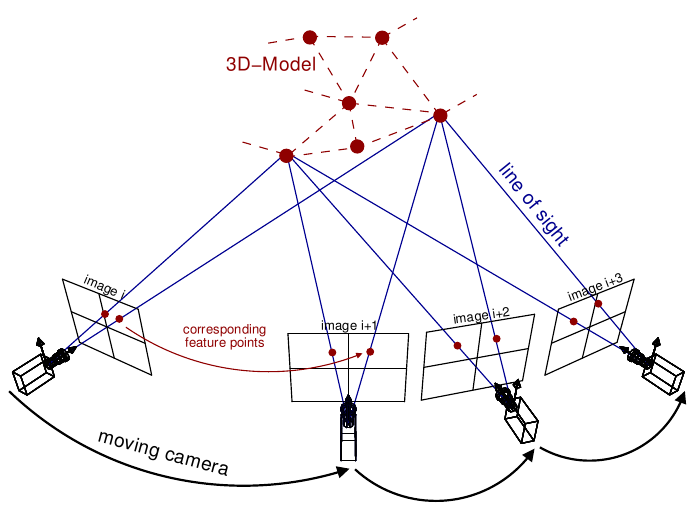
\includegraphics[width=0.45\textwidth]{sfm}
    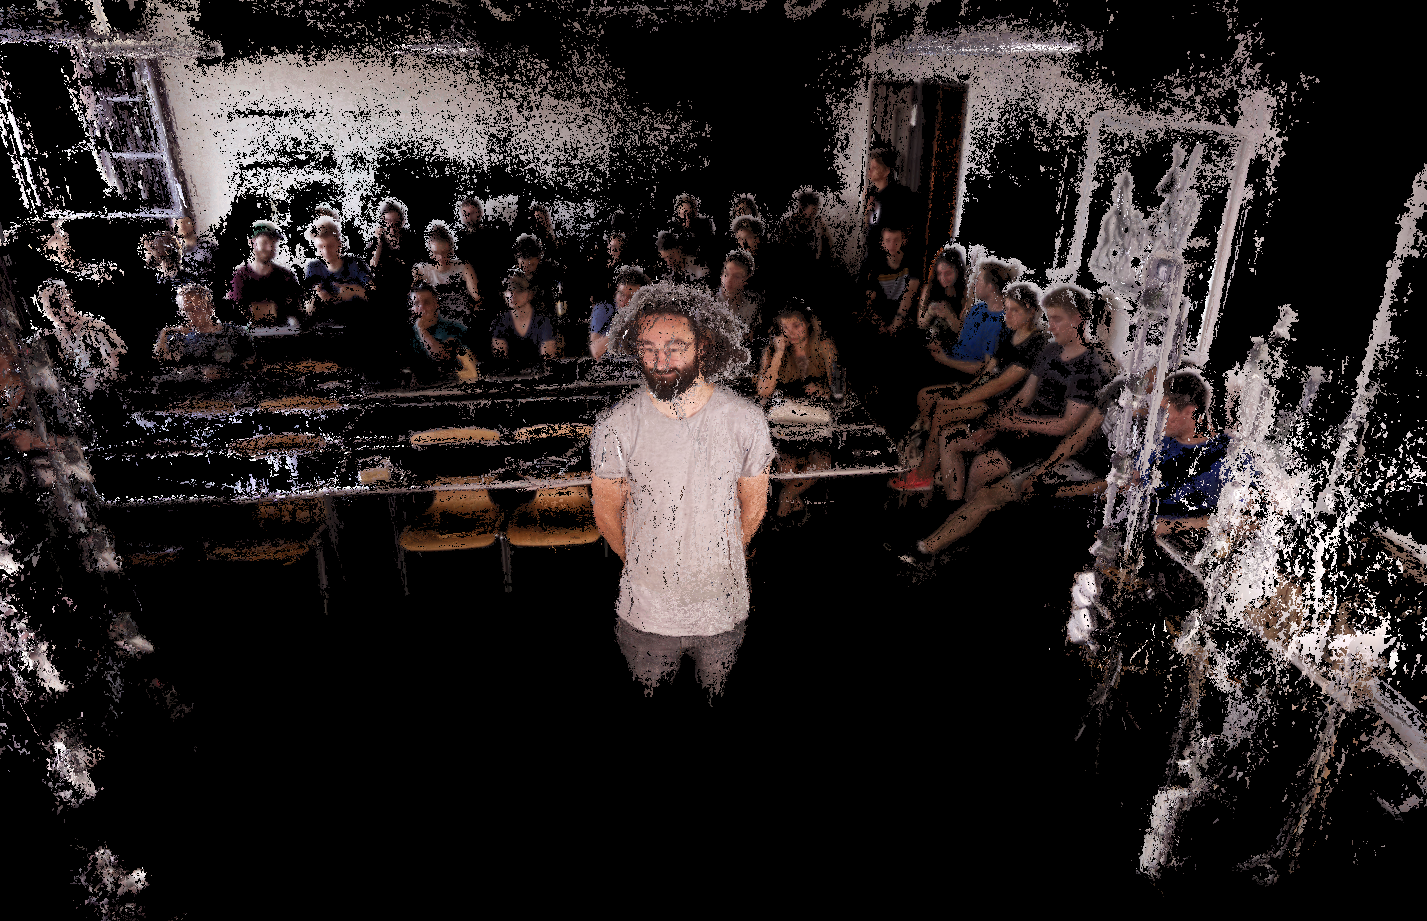
\includegraphics[width=0.45\textwidth]{depth_manu}
  \end{figure}

  \note{
    \begin{itemize}
      \item
      \item Image from \url{http://theia-sfm.org/}
    \end{itemize}
  }
\end{frame}


\begin{frame}{Optical Flow}

  \begin{figure}
    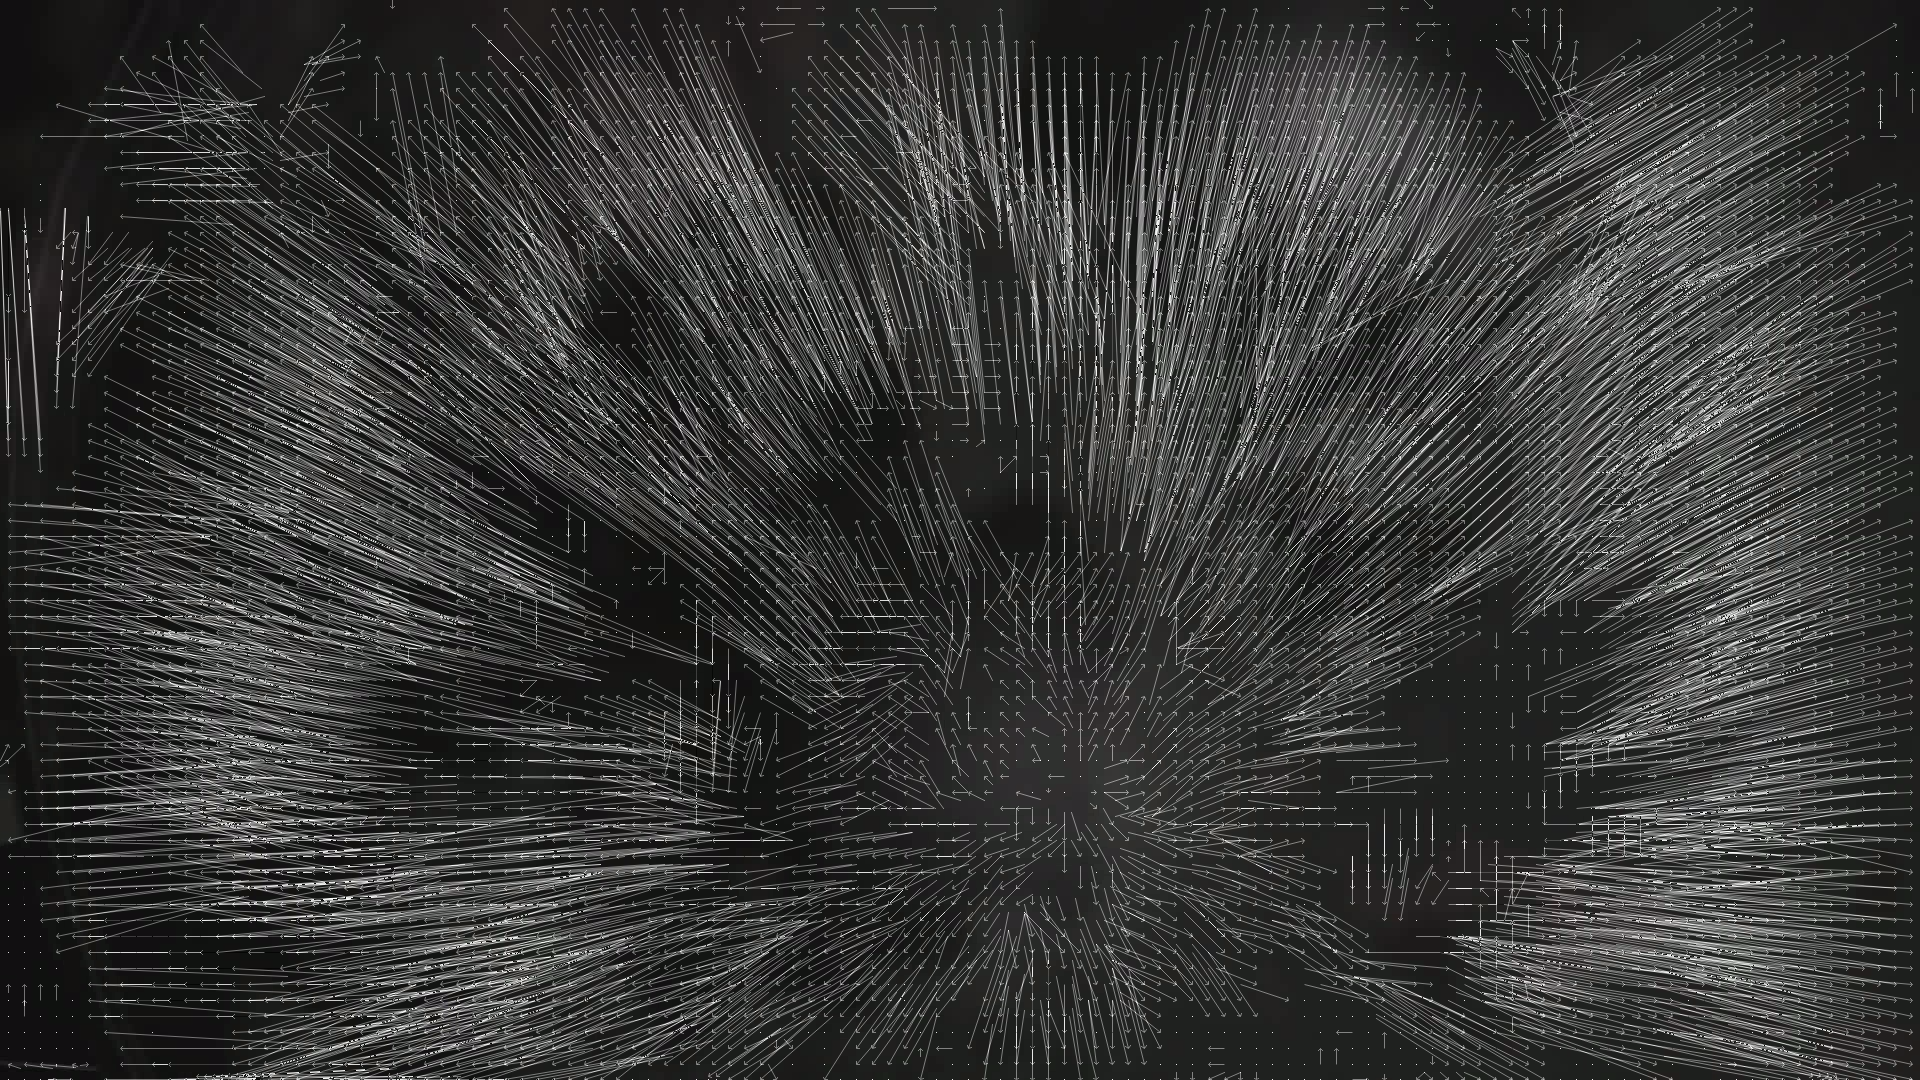
\includegraphics[height=0.45\textheight]{optical_flow_dense}
    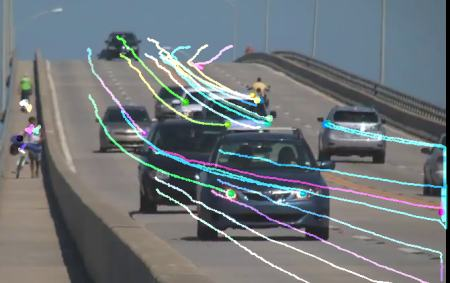
\includegraphics[height=0.45\textheight]{optical_flow_sparse}
  \end{figure}

  \note{
    \begin{itemize}
      \item Images from \url{https://de.wikipedia.org/wiki/Optischer_Fluss} and \url{https://docs.opencv.org/3.4/d4/dee/tutorial_optical_flow.html}
    \end{itemize}
  }
\end{frame}


\begin{frame}{State estimation}

  \begin{figure}
    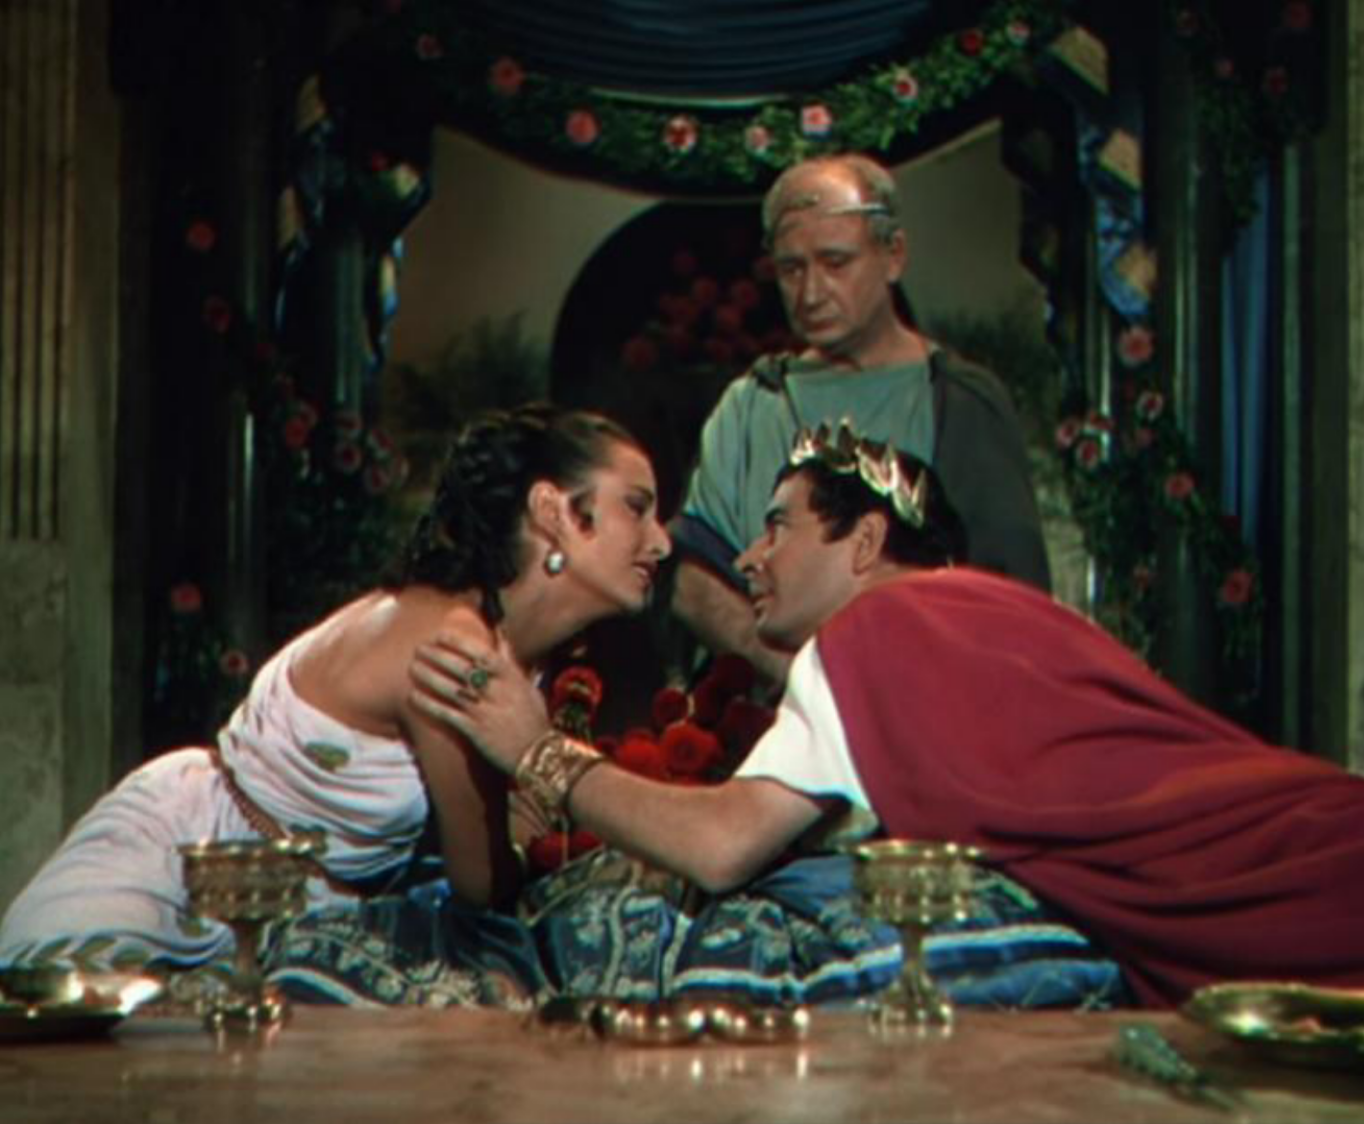
\includegraphics[width=0.65\textwidth]{quovadis}
  \end{figure}

  \note{
    \begin{itemize}
      \item Image from Quo Vadis, Action Recognition? A New Model and the Kinetics Dataset, Carreira \& Zissermann, NeurIPS 2014
      \item
    \end{itemize}
  }
\end{frame}


\begin{frame}{Semantic understanding of the world}

  \begin{figure}
    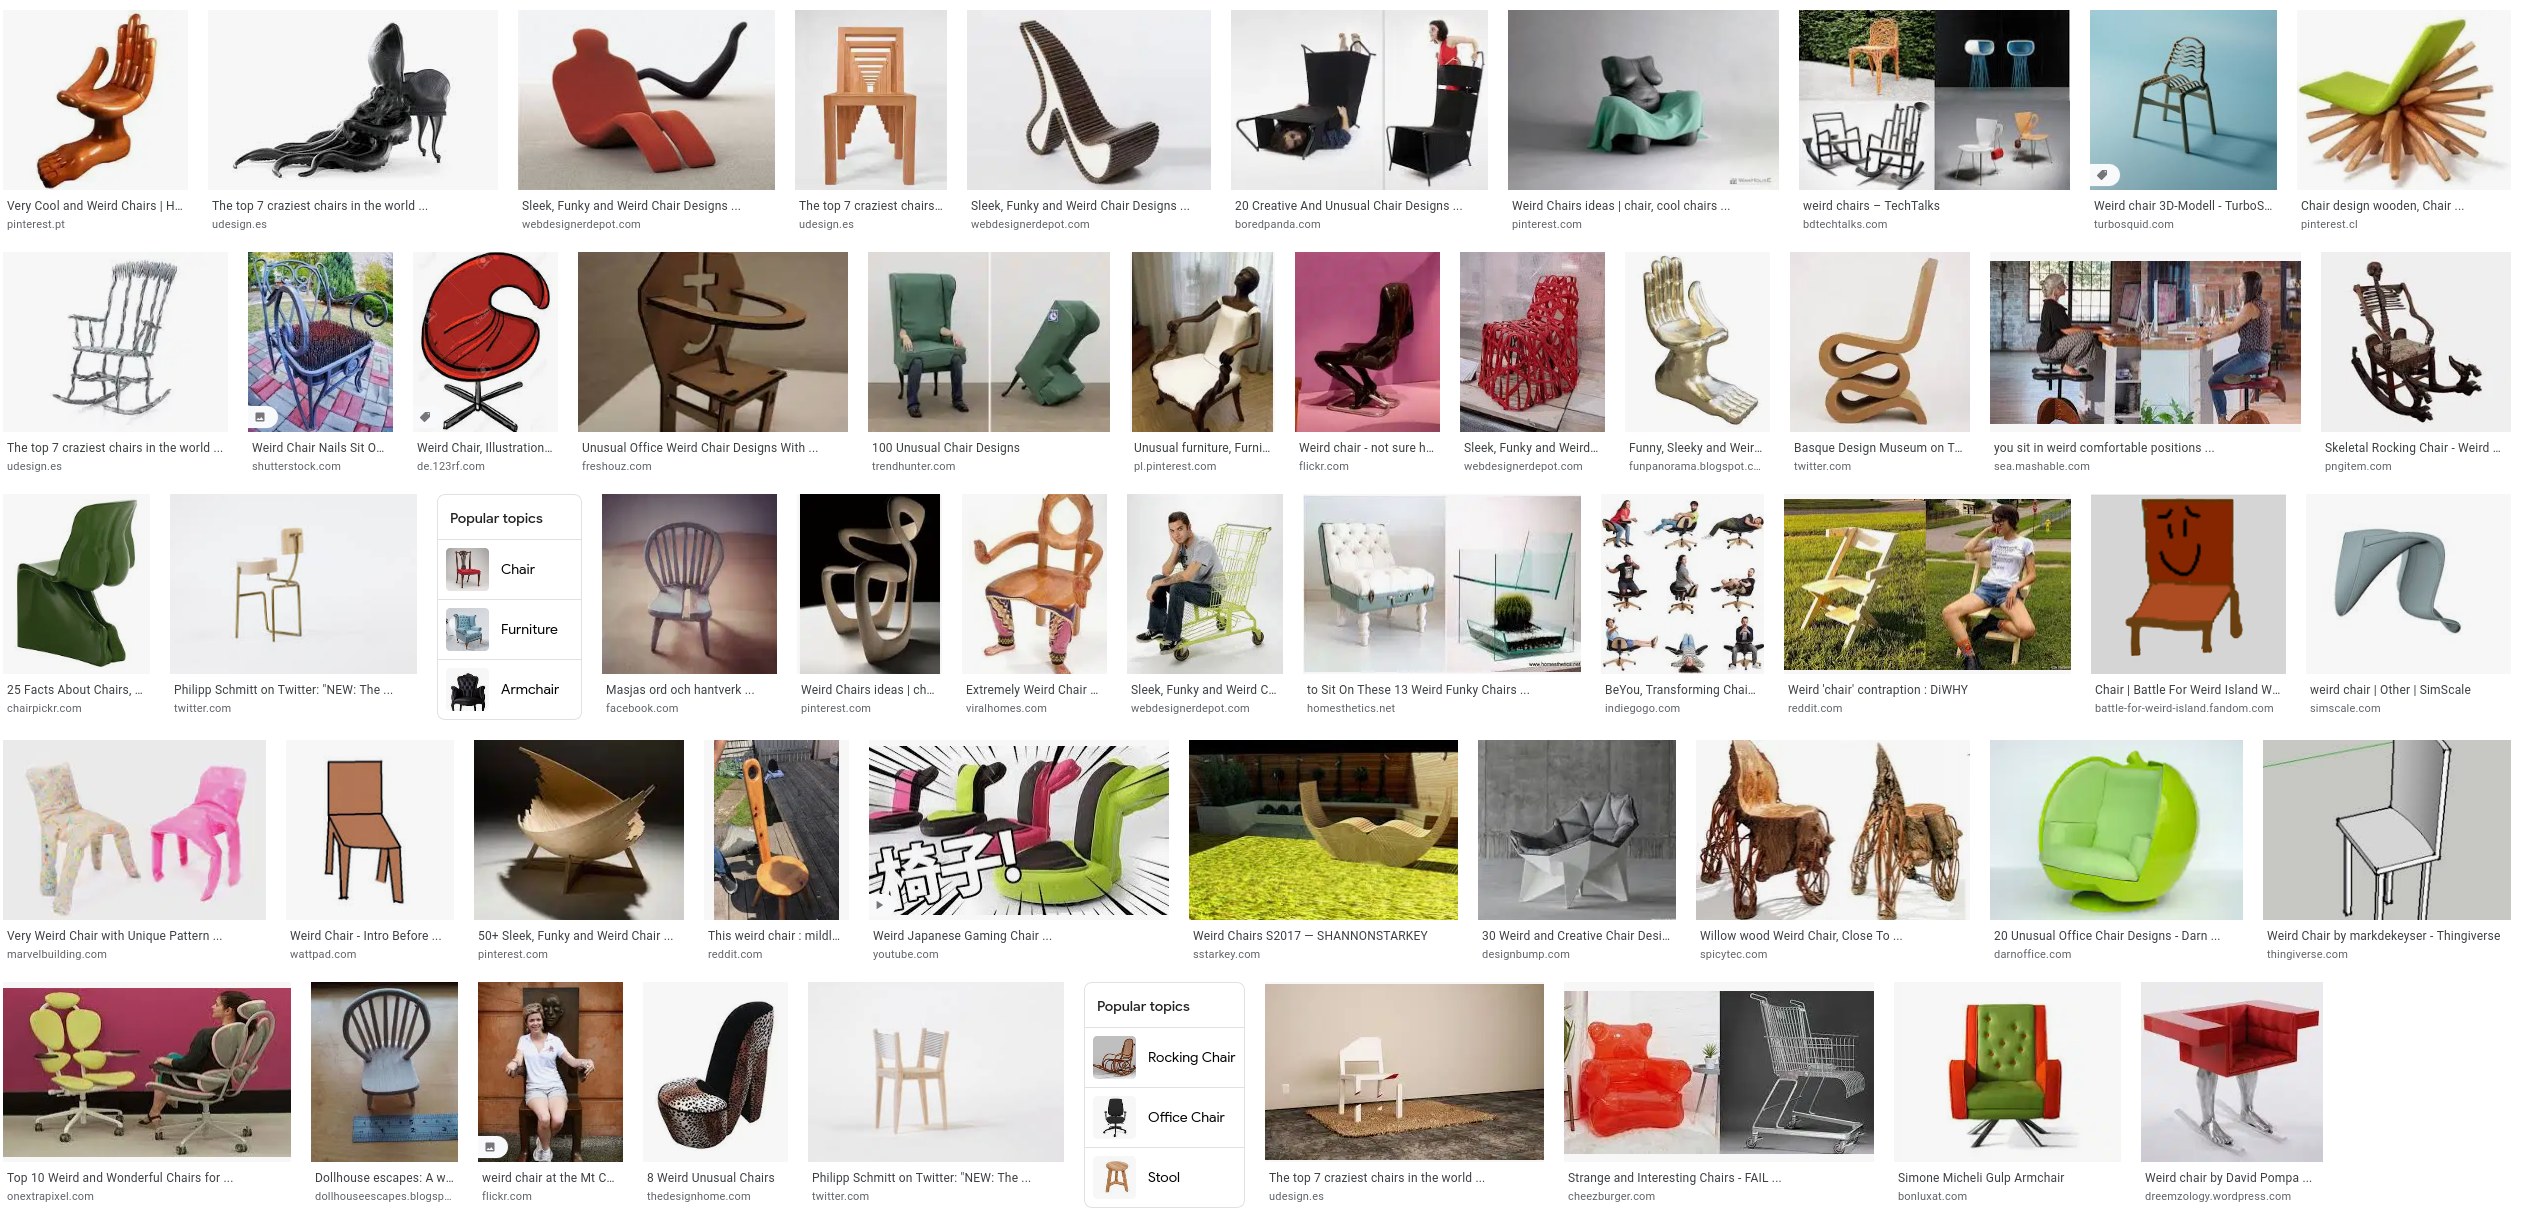
\includegraphics[width=0.95\textwidth]{weirdchairs}
  \end{figure}

  \note{
    \begin{itemize}
      \item Google image search for 'weird chairs'.
      \item
    \end{itemize}
  }
\end{frame}


\begin{frame}{Tasks}

  \begin{itemize}
    \item Action classification, Action detection
    \item Video captioning
    \item Object localization (position + orientation + dynamics)
    \item Forecasting
  \end{itemize}

\end{frame}


\begin{frame}{Datasets: UCF101}

  \begin{itemize}
    \item 13320 videos (YouTube)
    \item 101 action categories
  \end{itemize}

  \note{
    \begin{itemize}
      \item UCF101: A Dataset of 101 Human Action Classes From Videos in The Wild, Soomro et al., CRCV 2012
    \end{itemize}
  }

\end{frame}


\begin{frame}{Datasets: YouTube Sports 1M}

  \begin{itemize}
    \item 1,133,157 videos
    \item 487 sports classes
  \end{itemize}

  \note{
    \begin{itemize}
      \item Large-scale Video Classification with Convolutional Neural Networks, Karpathy et al., CVPR 2014
    \end{itemize}
  }

\end{frame}


\begin{frame}{Datasets: Atomic Visual Actions (AVA) v2}

  \begin{itemize}
    \item 80 atomic visual actions
    \item 430 15-minute movie clips
    \item 1.62M action labels (bounding boxes in space and time)
  \end{itemize}

  \note{
    \begin{itemize}
      \item Hollywood in Homes: Crowdsourcing Data Collection for Activity Understanding, Gunnar et al., ECCV 2016
      \item AVA: A Video Dataset of Spatio-temporally Localized Atomic Visual Actions, Gu et al., CVPR 2018
    \end{itemize}
  }

\end{frame}


\begin{frame}{Datasets: Kinetics 400/600/700}

  \begin{itemize}
    \item 650000 video clips
    \item 400/600/700 action classes
  \end{itemize}

  \note{
    \begin{itemize}
      \item A Short Note on the Kinetics-700-2020 Human Action Dataset, Smaira et al., 2020
    \end{itemize}
  }

\end{frame}


\begin{frame}{Video Analysis}

  What are the challenges?

\end{frame}


\begin{frame}{Video Analysis}

  What are the challenges?

    \begin{itemize}
      \item More data, higher redundancy
      \item Lower quality (resolution, motion)
      \item Higher variance
    \end{itemize}

\end{frame}



\begin{frame}{Video Analysis}

  How could we analyze videos?

\end{frame}


\begin{frame}{Fusion}

  \begin{figure}
    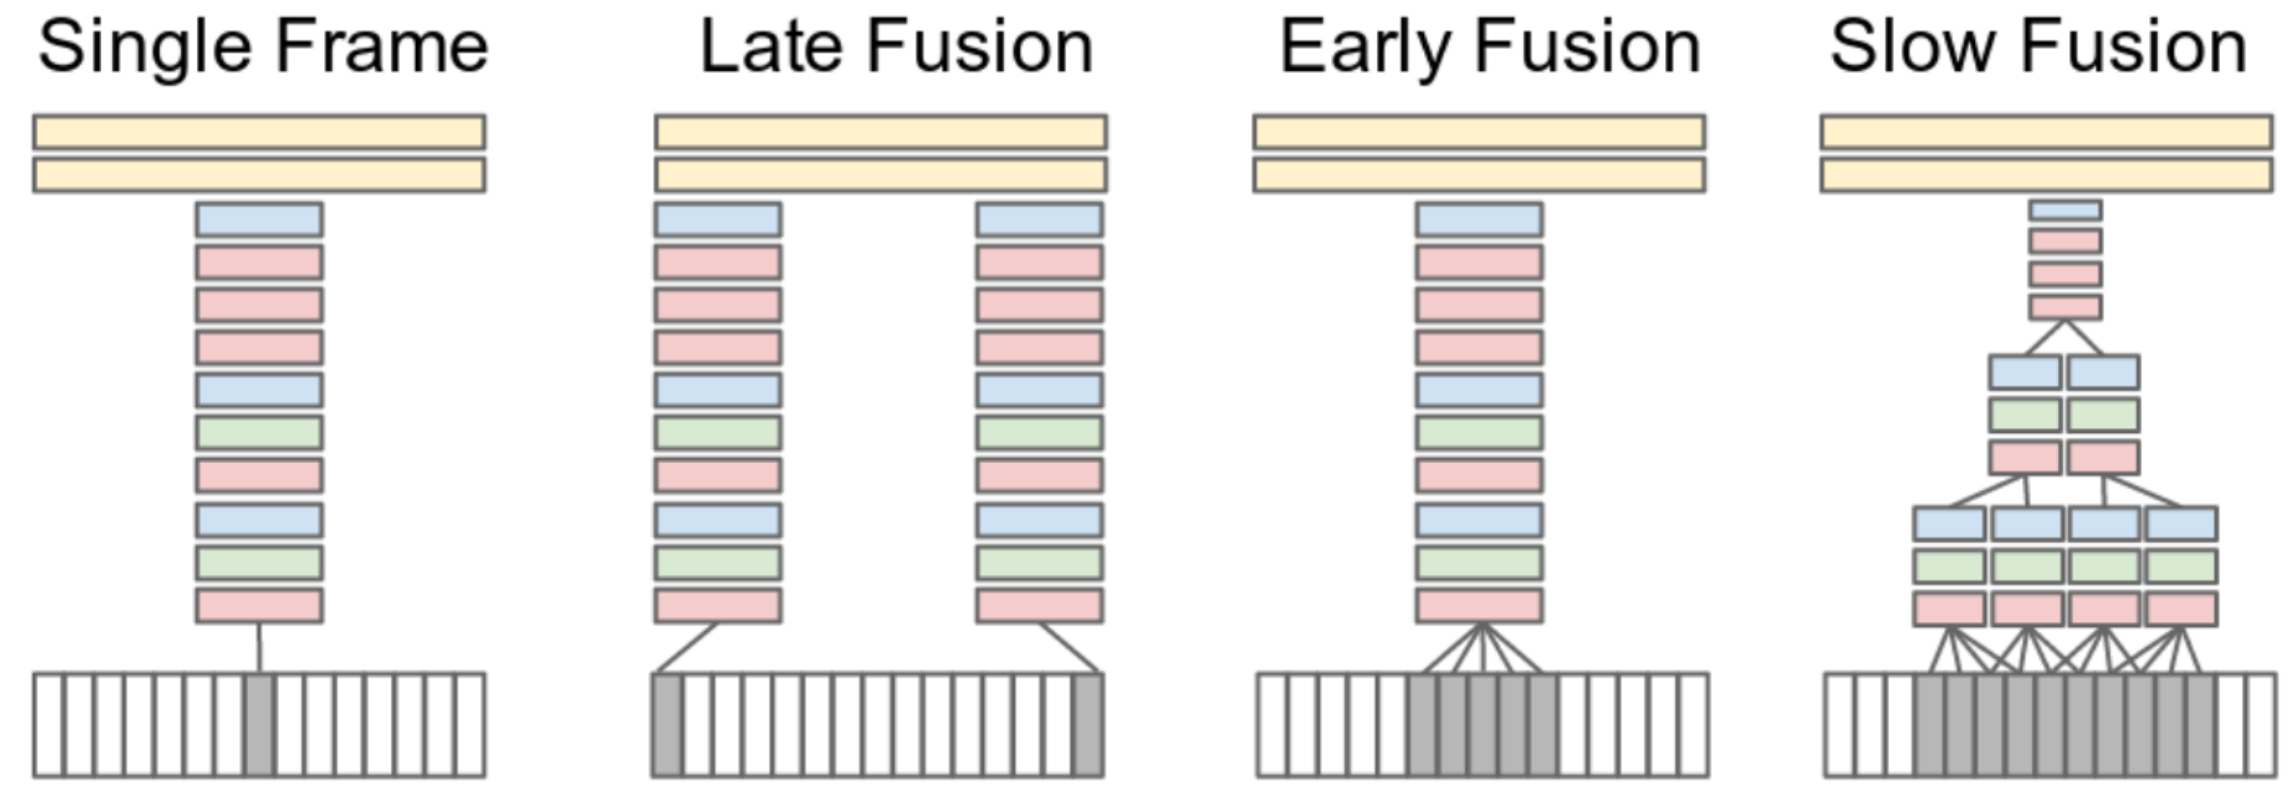
\includegraphics[width=0.85\textwidth]{fusion_00}
  \end{figure}

  \note{
    \begin{itemize}
      \item Information along the time domain can be integrated on different levels of abstraction.
      \item Image from Large-scale Video Classification with Convolutional Neural Networks, Karpathy et al, CVPR 2014
    \end{itemize}
  }
\end{frame}


\begin{frame}{Two-stream architectures}

  \begin{figure}
    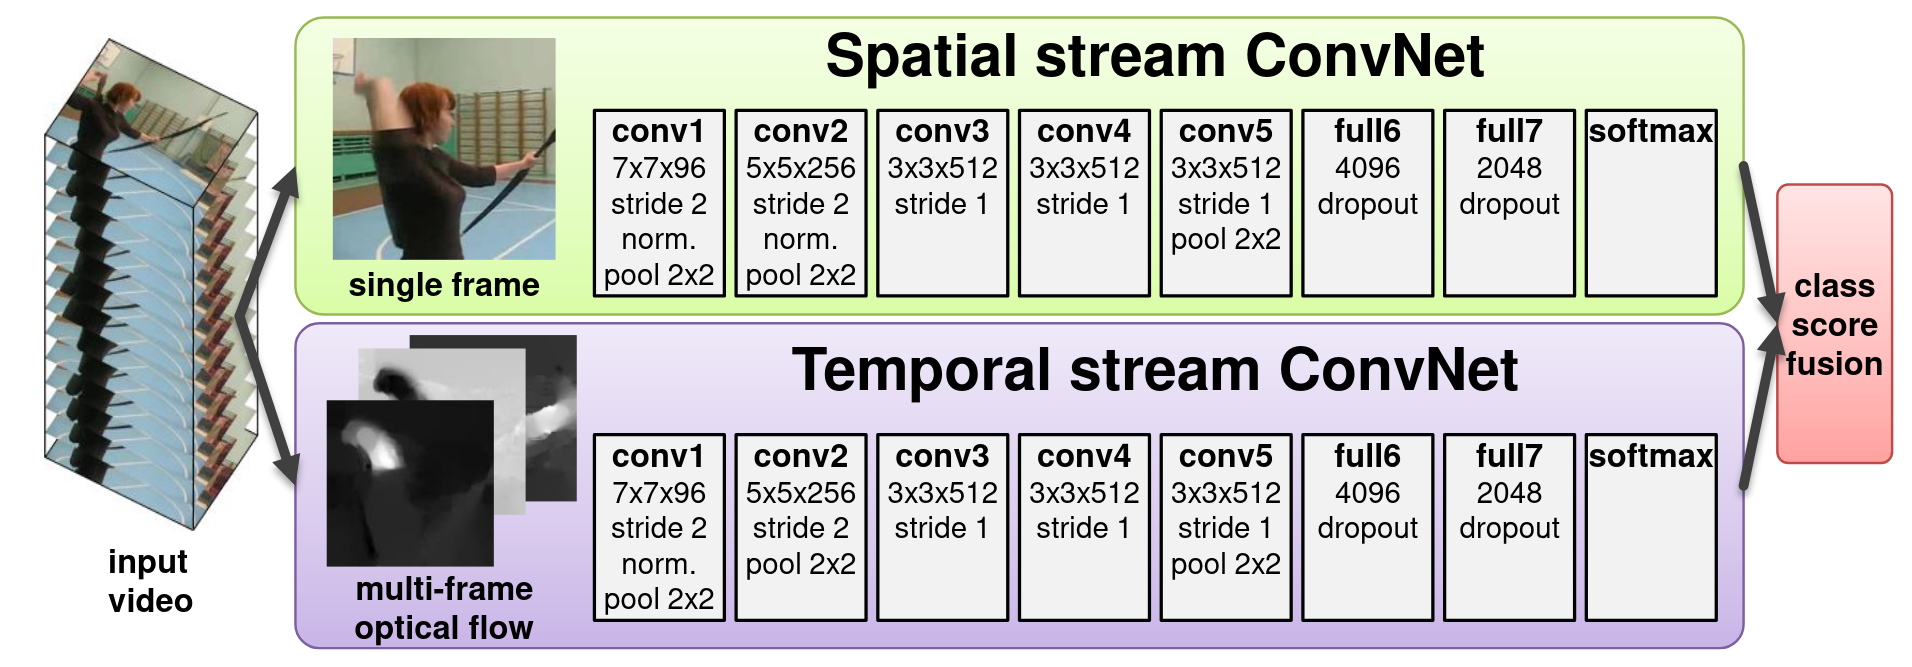
\includegraphics[width=0.85\textwidth]{twostream}
  \end{figure}

  \note{
    \begin{itemize}
      \item Inspired by the two-stream hypothesis (dorsal stream: where, ventral stream what) \\ \url{https://en.wikipedia.org/wiki/Two-streams_hypothesis}
      \item Image from Two-Stream Convolutional Networks for Action Recognition in Videos, Simonyan \& Zissermann, NeurIPS 2014
    \end{itemize}
  }
\end{frame}


\begin{frame}{Inflated 3D CNNs (I3D)}

    \begin{itemize}
      \item Build 3D Convolutional Neural Networks based on well known architectures
      \item Initialize weights with networks pre-trained on ImageNet
      \item Replicate weights as if network is applied to boring video \\ (sequence of duplicates of single frame)
      \item Striding and pooling have to be adjusted for time domain
    \end{itemize}

  \note{
    \begin{itemize}
      \item Quo Vadis, Action Recognition? A New Model and the Kinetics Dataset, Carreira \& Zissermann, CVPR 2017
    \end{itemize}
  }
\end{frame}


\begin{frame}{Two-stream Inflated 3D CNNs (I3D)}

  \begin{figure}
    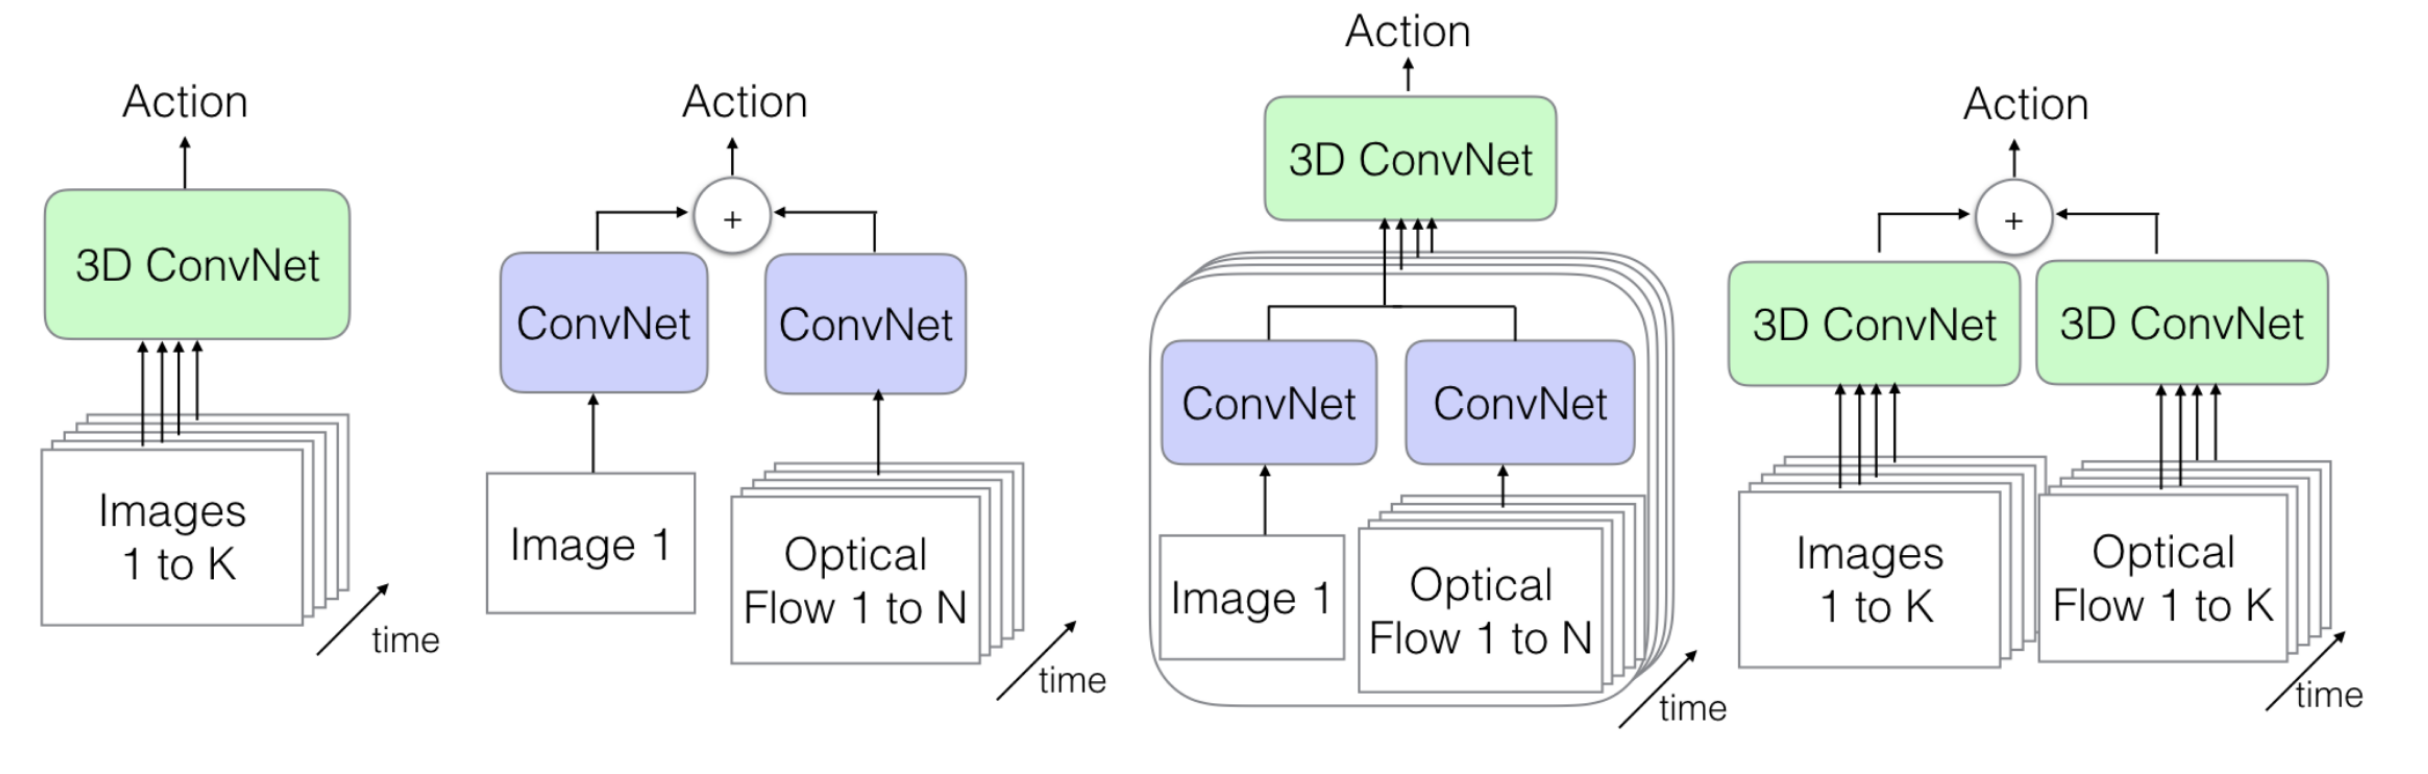
\includegraphics[width=0.85\textwidth]{twostream_i3d}
  \end{figure}

  \note{
    \begin{itemize}
      \item Even with 3d convolutional networks a second steam based on optical flow improves the results.
      \item Image from Quo Vadis, Action Recognition? A New Model and the Kinetics Dataset, Carreira \& Zissermann, CVPR 2017
    \end{itemize}
  }
\end{frame}


\begin{frame}{SlowFast}

  \begin{figure}
    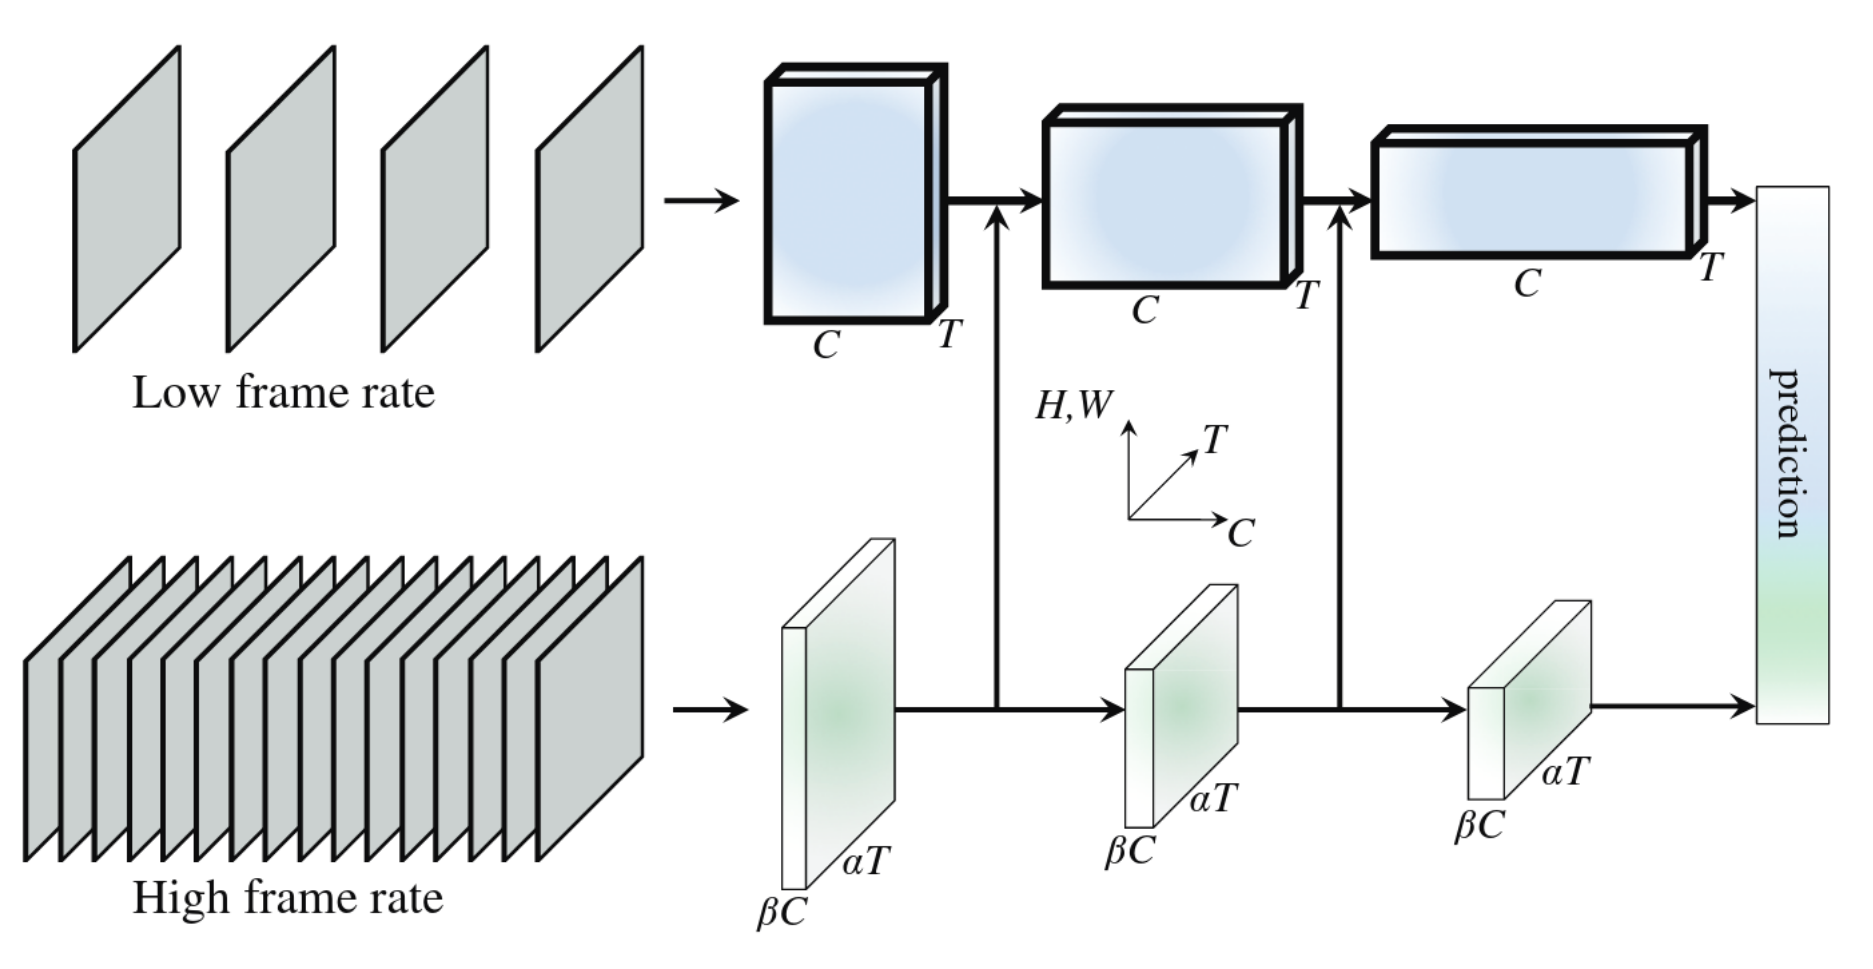
\includegraphics[width=0.65\textwidth]{slowfast}
  \end{figure}

  \note{
    \begin{itemize}
      \item Inspired by the retinal ganglion cells.
      \item $80\%$ of computation for low frame rate but high spatial resolution
      \item $20\%$ of computation for high temporal resolution but less spatial detail and lower dimensionality (channels)
      \item SlowFast Networks for Video Recognition, Feichtenhofer et al., ICCV 2019
    \end{itemize}
  }
\end{frame}


\begin{frame}{Tube-CNN}

  \begin{figure}
    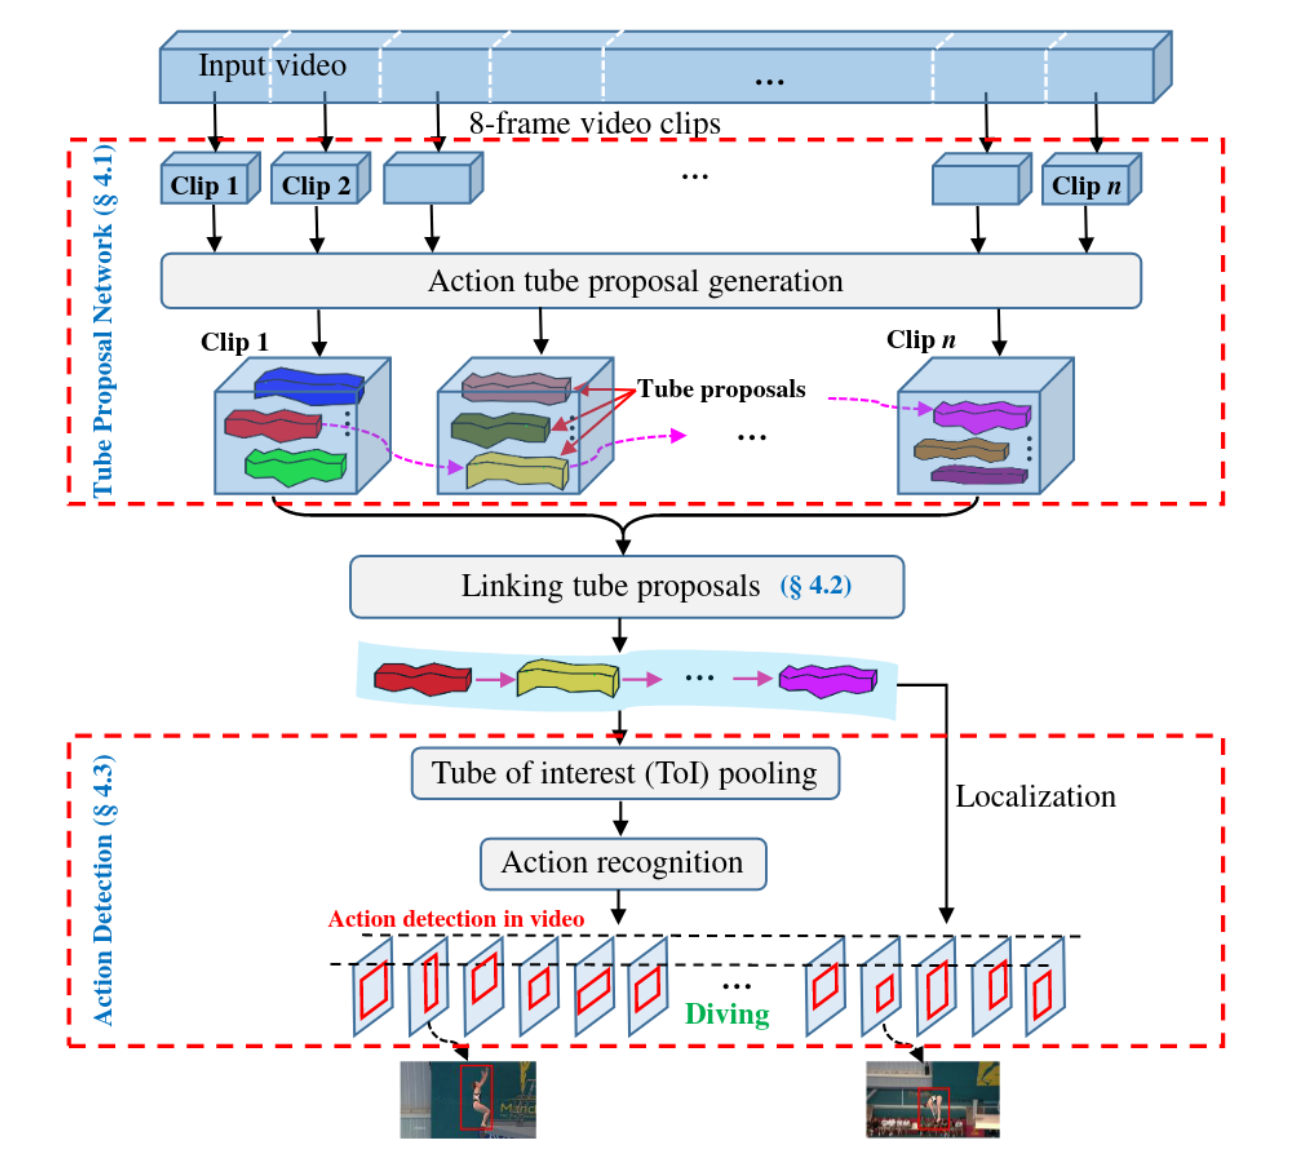
\includegraphics[height=0.95\textheight]{tube_cnn}
  \end{figure}

  \note{
    \begin{itemize}
      \item Extending Faster R-CNN to the time domain for action localization.
      \item Tube Convolutional Neural Network (T-CNN) for Action Detection in Videos, Hou et al., ICCV 2017
    \end{itemize}
  }
\end{frame}


\begin{frame}{Tube-CNN}

  \begin{figure}
    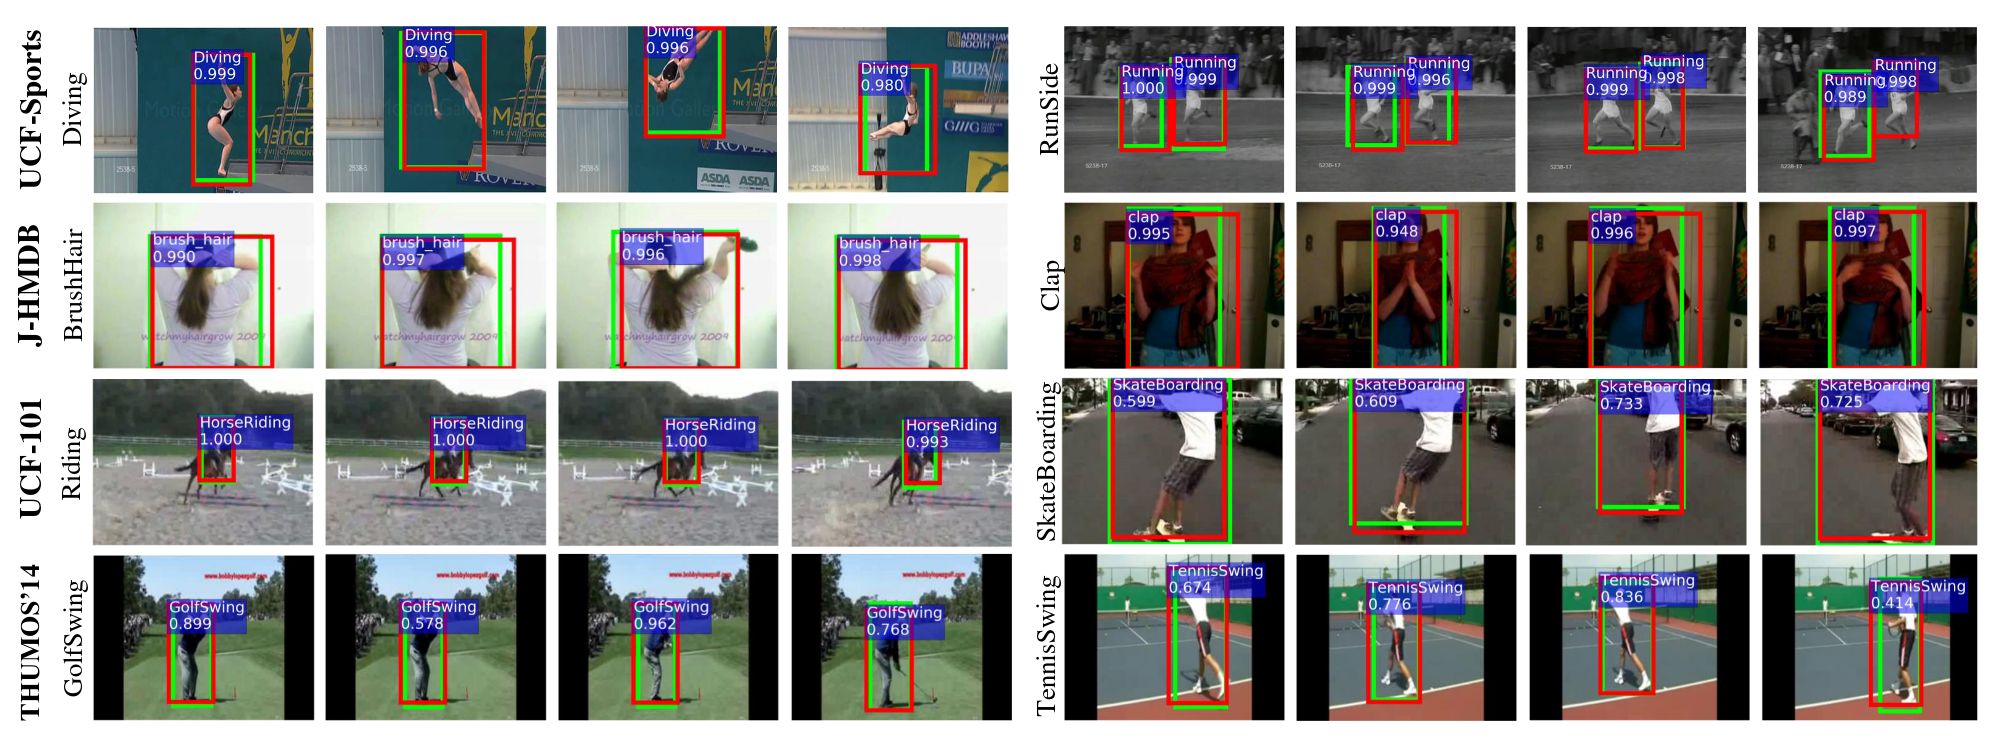
\includegraphics[width=0.95\textwidth]{tube_cnn_result}
  \end{figure}

  \note{
    \begin{itemize}
      \item Tube Convolutional Neural Network (T-CNN) for Action Detection in Videos, Hou et al., ICCV 2017
    \end{itemize}
  }
\end{frame}




\begin{frame}{Recurrent Neural Networks}

    \begin{itemize}
      \item So far we modeled time/sequences with feed forward networks
      \item What if we want to have long input sequences?
      \item What if the interpretation of the next input is dependent on the previous input?
    \end{itemize}

\end{frame}


\begin{frame}{Recurrent Neural Networks}

  \begin{figure}
    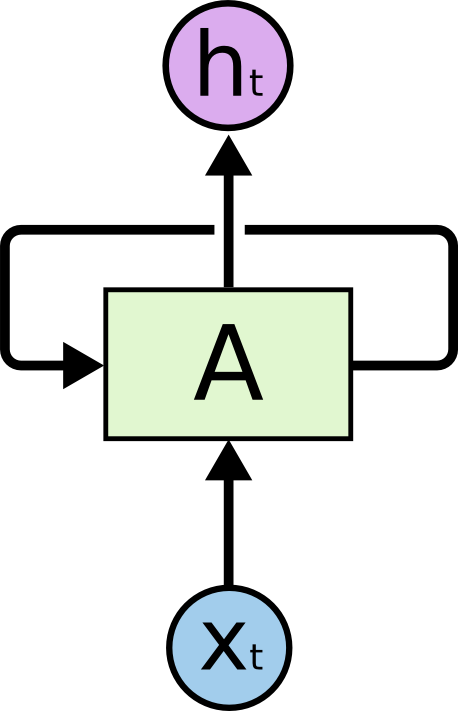
\includegraphics[height=0.85\textheight]{rnn_00}
  \end{figure}

  \note{
    \begin{itemize}
      \item A recurrent neural network is a network with a loop.
      \item Image from Understanding LSTM Networks, Chris Olah\\
            \url{https://colah.github.io/posts/2015-08-Understanding-LSTMs/}
    \end{itemize}
  }
\end{frame}


\begin{frame}{Recurrent Neural Networks}

  \begin{figure}
    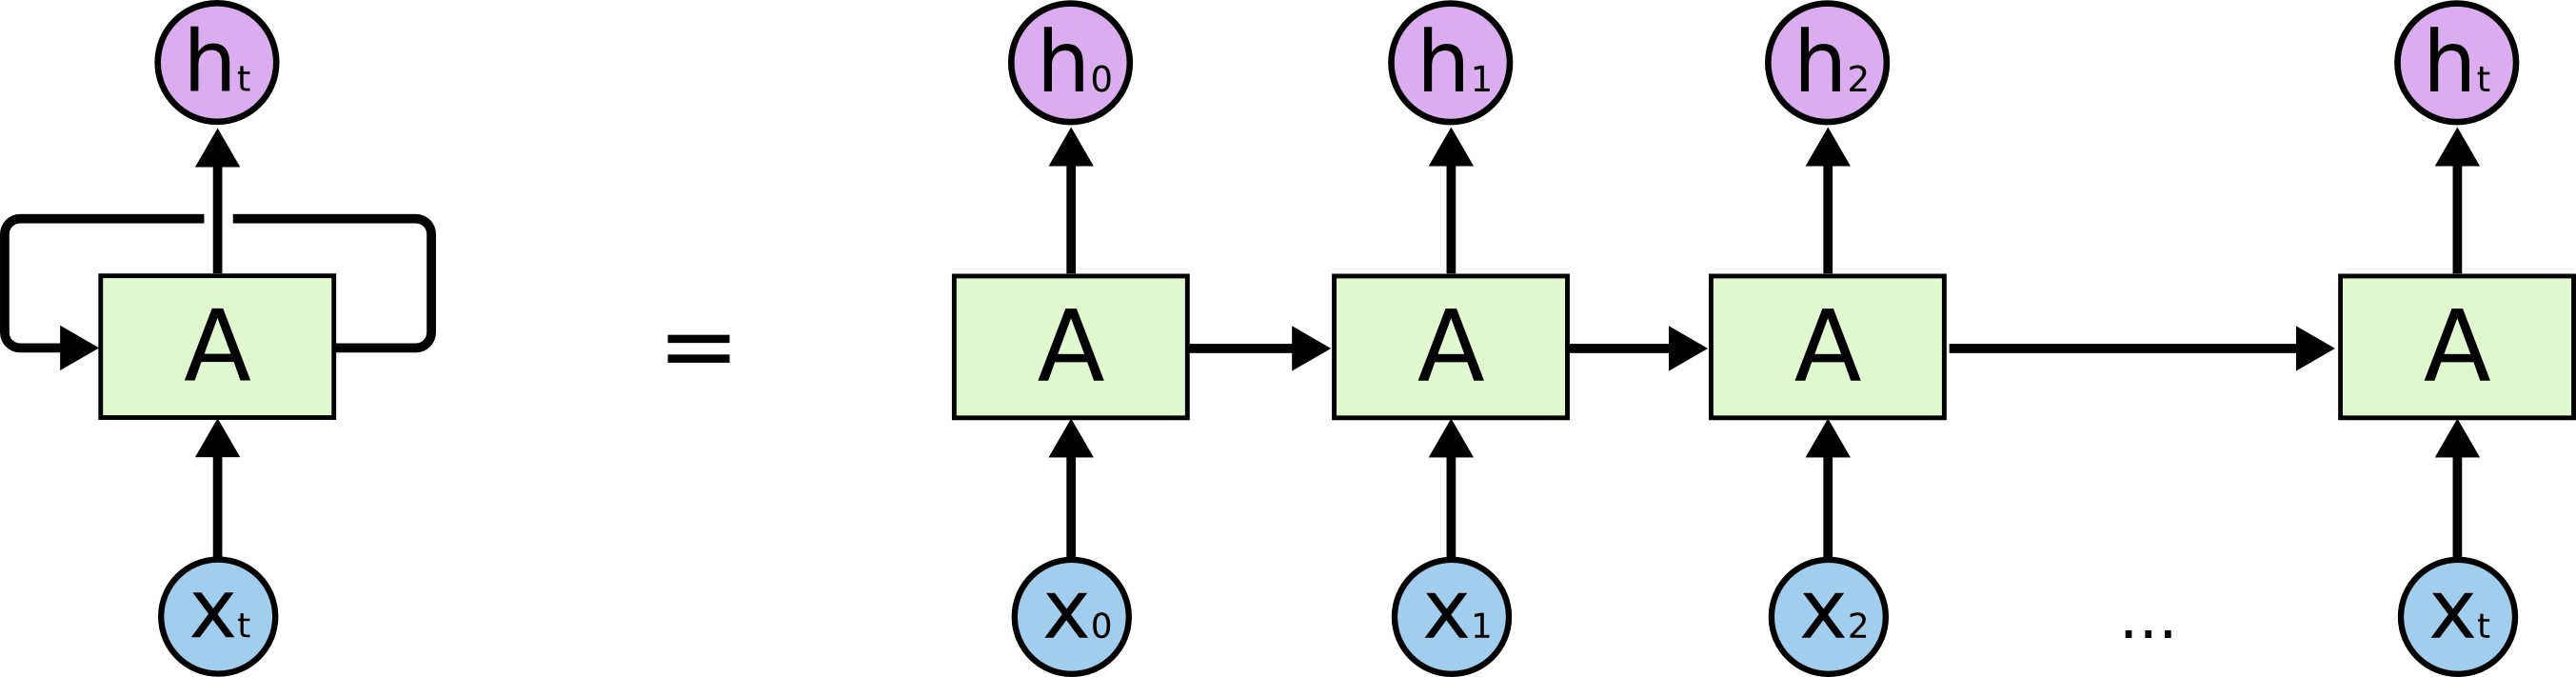
\includegraphics[width=0.85\textwidth]{rnn_01}
  \end{figure}

  \note{
    \begin{itemize}
      \item
      \item Image from Understanding LSTM Networks, Chris Olah\\
            \url{https://colah.github.io/posts/2015-08-Understanding-LSTMs/}
    \end{itemize}
  }
\end{frame}



\begin{frame}{Recurrent Neural Networks}

  \begin{figure}
    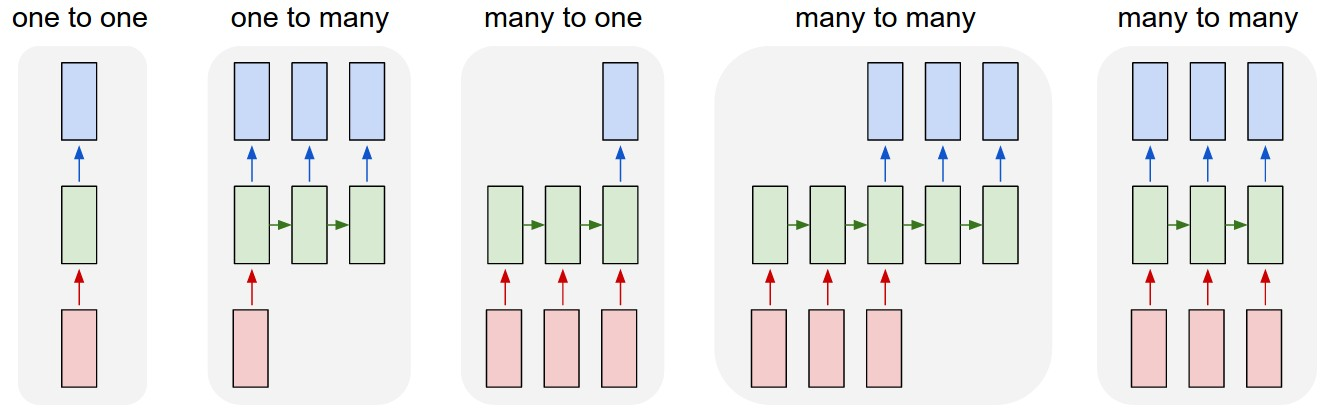
\includegraphics[width=0.85\textwidth]{rnn_in_out}
  \end{figure}

  \note{
    \begin{itemize}

      \item Image from The Unreasonable Effectiveness of Recurrent Neural Networks, Andrej Karpathy\\
            \url{https://karpathy.github.io/2015/05/21/rnn-effectiveness/}
    \end{itemize}
  }
\end{frame}


\begin{frame}{RNN: Backprop through time}

  \begin{figure}
    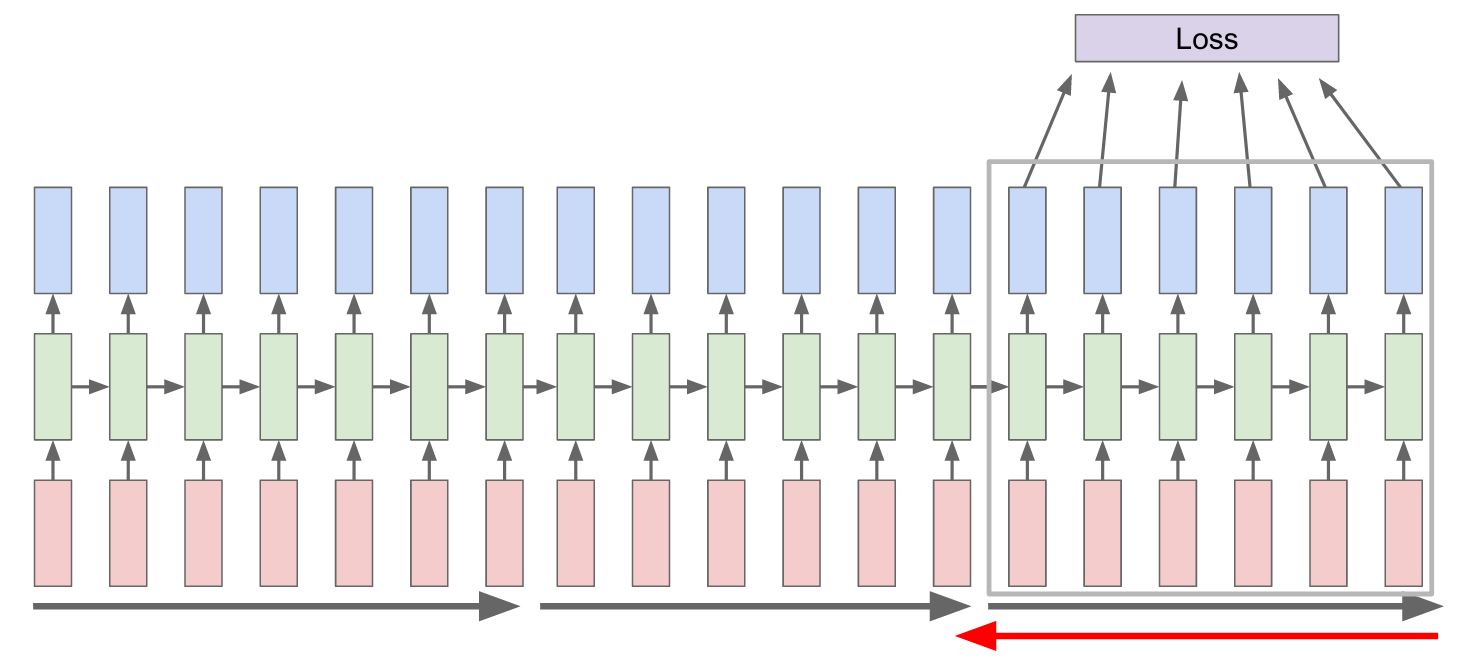
\includegraphics[width=0.85\textwidth]{truncatedbackprop}
  \end{figure}

  \note{
    \begin{itemize}
      \item
      \item Image from Stanford CS231n Lecture 10, Fei-Fei Li \url{http://cs231n.stanford.edu/slides/2021/lecture_10.pdf}
    \end{itemize}
  }
\end{frame}


\begin{frame}{RNN: Backprop through time}

  RNNs are cool because,
  \begin{itemize}
    \item they can process any length input,
    \item for processing input at $t$ they can use information from $t-k$,
    \item model size does not increase with sequence length,
  \end{itemize}
  but
  \begin{itemize}
    \item What information should be saved in the state? For how long?
    \item Recursive term in gradient: vanishing/exploding gradients
  \end{itemize}

\end{frame}


\begin{frame}{Long Short Term Memory Networks}

  \begin{figure}
    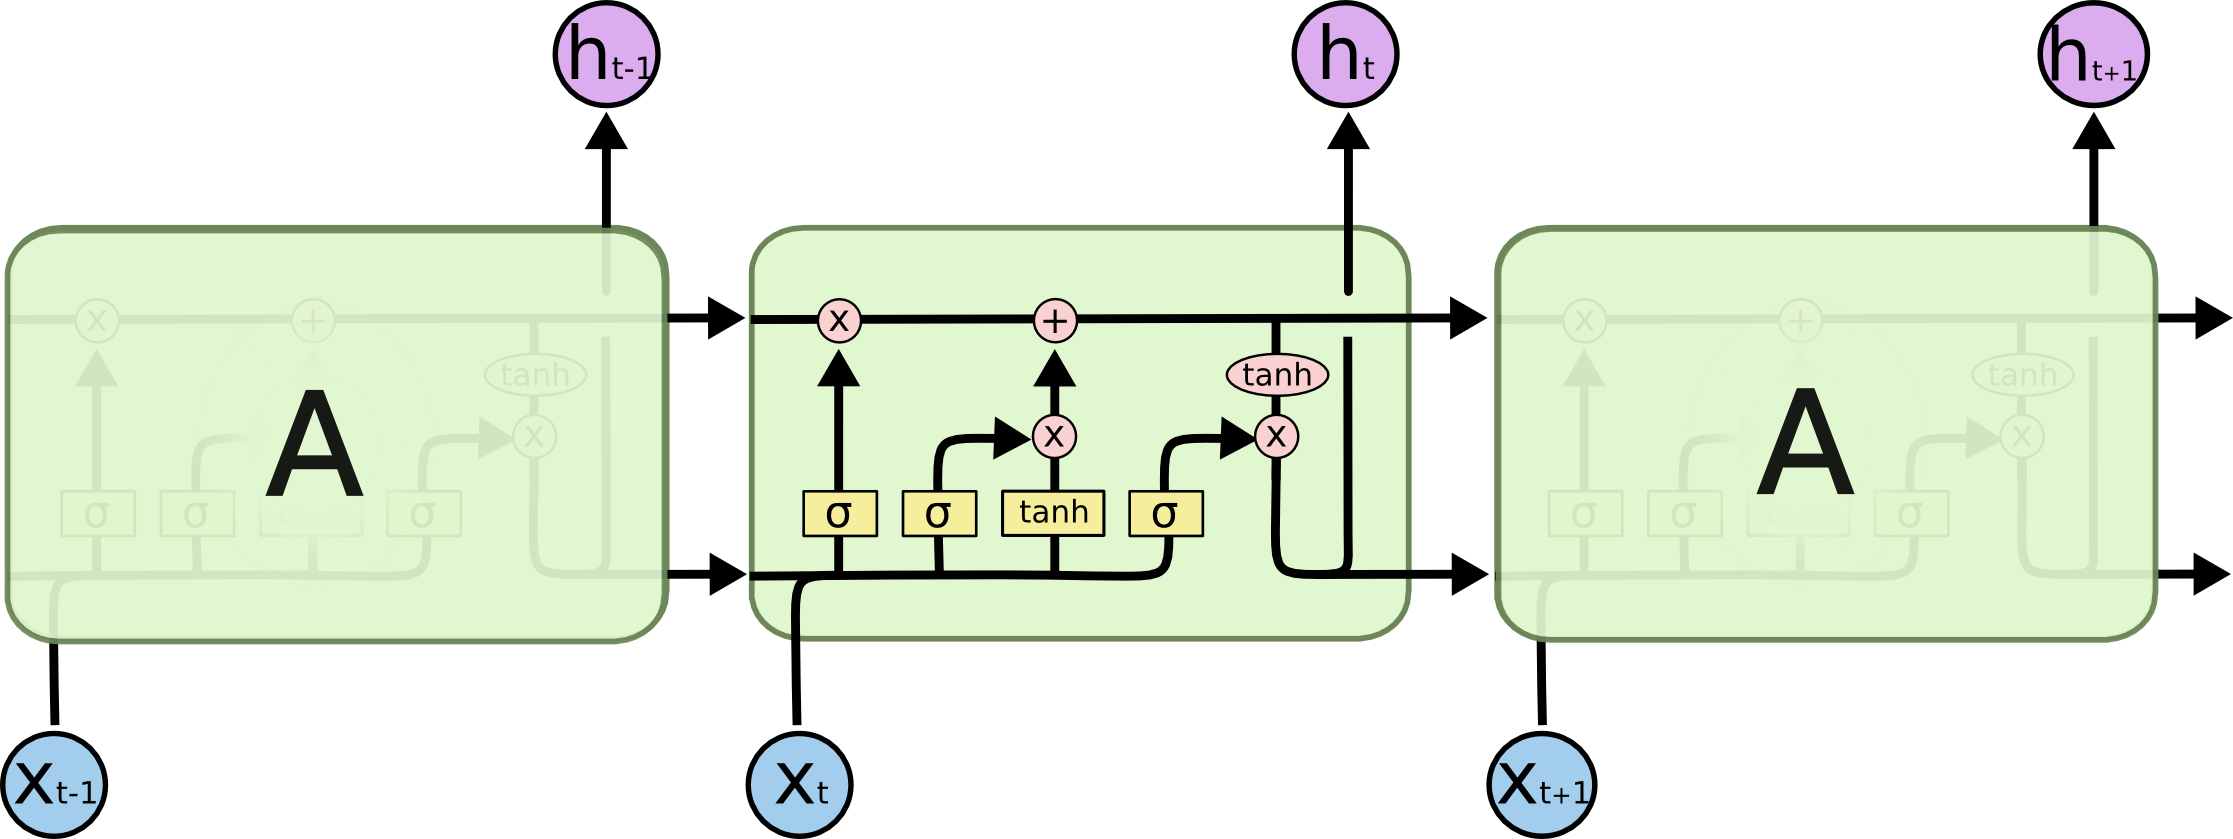
\includegraphics[width=0.85\textwidth]{rnn_lstm_full}
  \end{figure}

  \note{
    \begin{itemize}
      \item Long Short-Term Memory, Hochreiter \& Schmidhuber, 1997
      \item Image from Understanding LSTM Networks, Chris Olah\\
            \url{https://colah.github.io/posts/2015-08-Understanding-LSTMs/}
    \end{itemize}
  }
\end{frame}


\begin{frame}{Long Short Term Memory Networks}

  \begin{figure}
    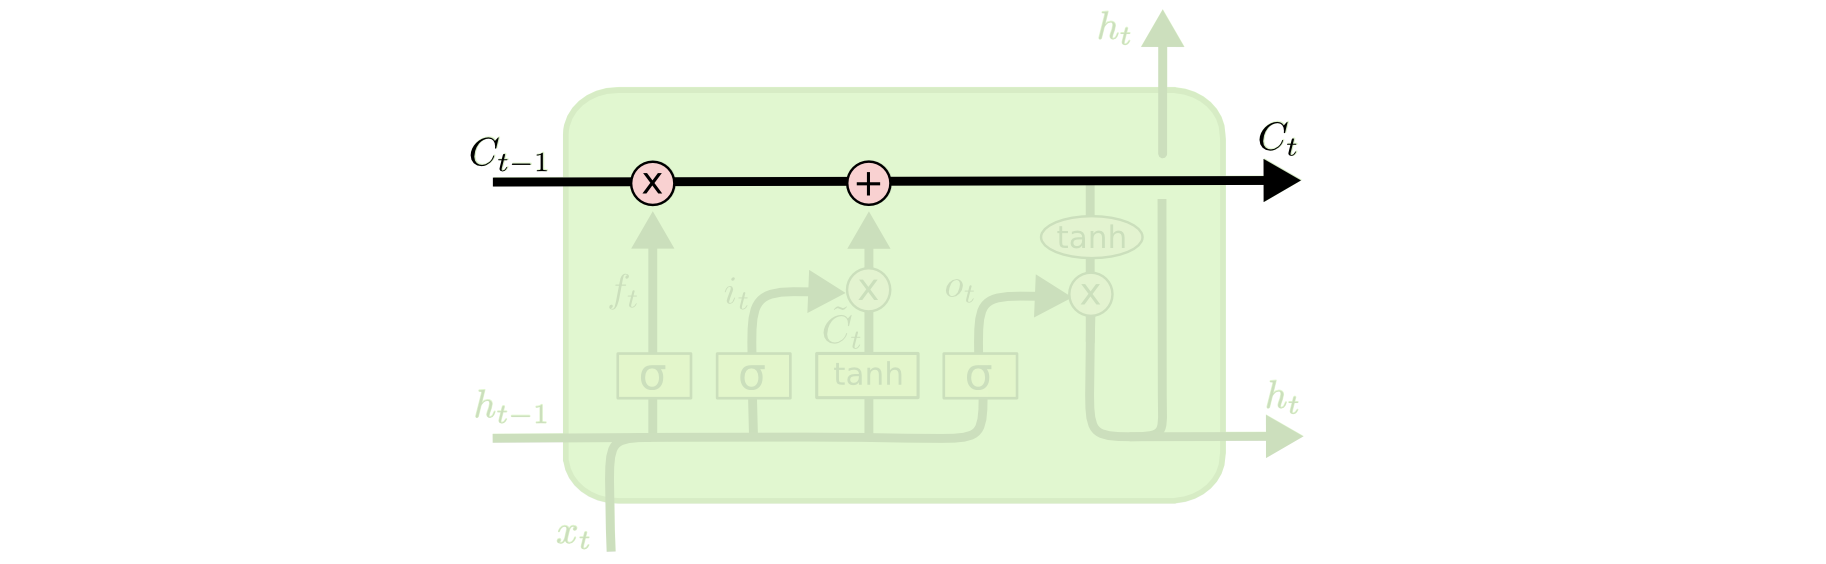
\includegraphics[width=0.85\textwidth]{rnn_lstm_00}
  \end{figure}

  \note{
    \begin{itemize}
      \item LSTMs have a cell state, that allows to store information.
      \item Image from Understanding LSTM Networks, Chris Olah\\
            \url{https://colah.github.io/posts/2015-08-Understanding-LSTMs/}
    \end{itemize}
  }
\end{frame}


\begin{frame}{Long Short Term Memory Networks}

  \begin{figure}
    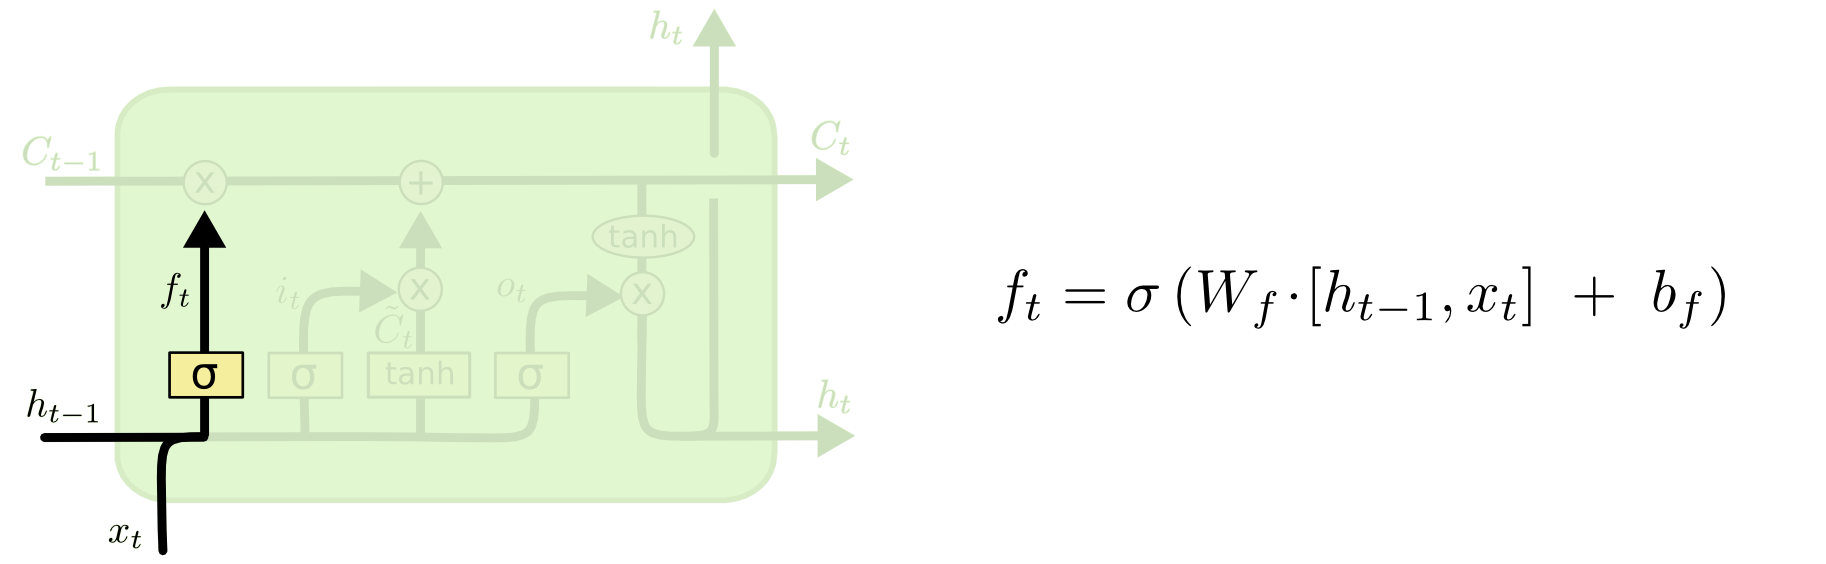
\includegraphics[width=0.85\textwidth]{rnn_lstm_01}
  \end{figure}

  \note{
    \begin{itemize}
      \item The forget gate allows to delete content from the cell state.
      \item Image from Understanding LSTM Networks, Chris Olah\\
            \url{https://colah.github.io/posts/2015-08-Understanding-LSTMs/}
    \end{itemize}
  }
\end{frame}


\begin{frame}{Long Short Term Memory Networks}

  \begin{figure}
    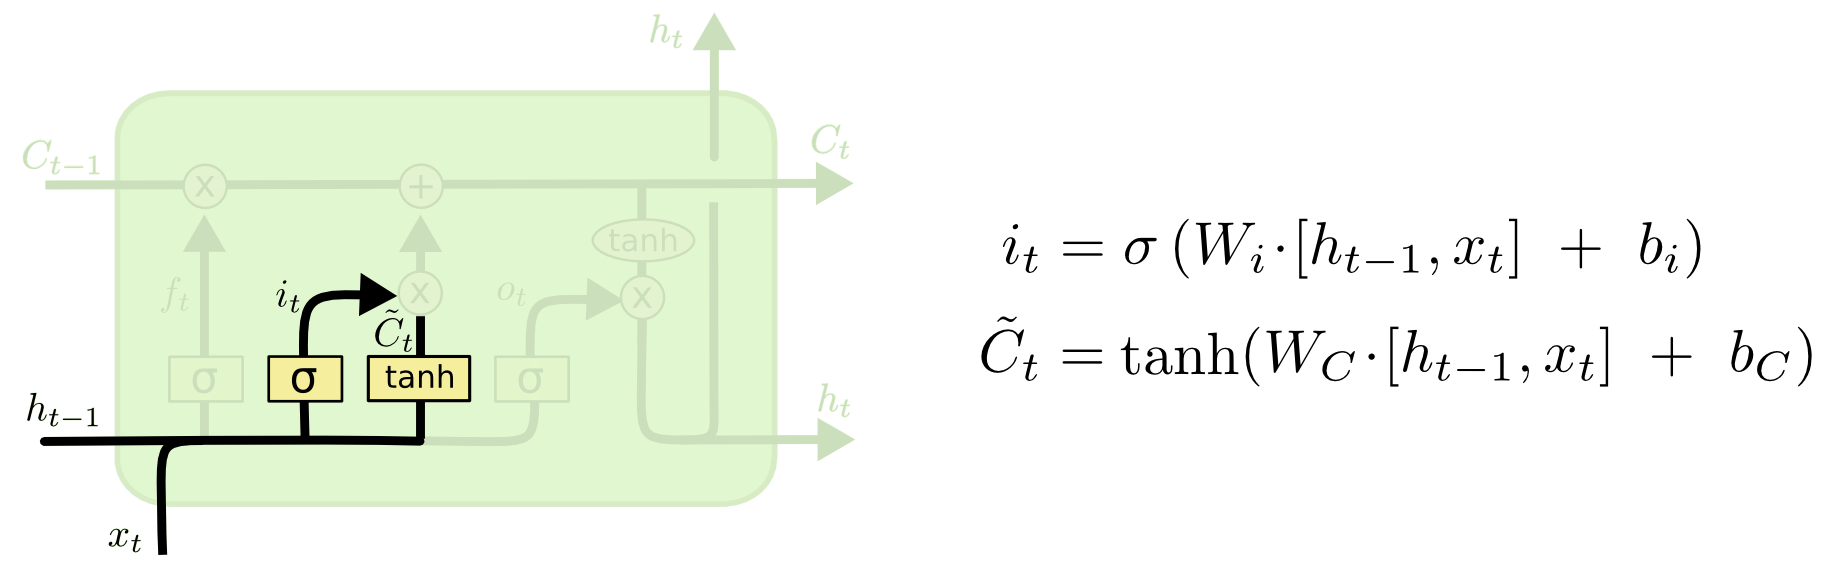
\includegraphics[width=0.85\textwidth]{rnn_lstm_02}
  \end{figure}

  \note{
    \begin{itemize}
      \item The input gate decides which parts of a new candidate state are written to the cell state.
      \item Image from Understanding LSTM Networks, Chris Olah\\
            \url{https://colah.github.io/posts/2015-08-Understanding-LSTMs/}
    \end{itemize}
  }
\end{frame}


\begin{frame}{Long Short Term Memory Networks}

  \begin{figure}
    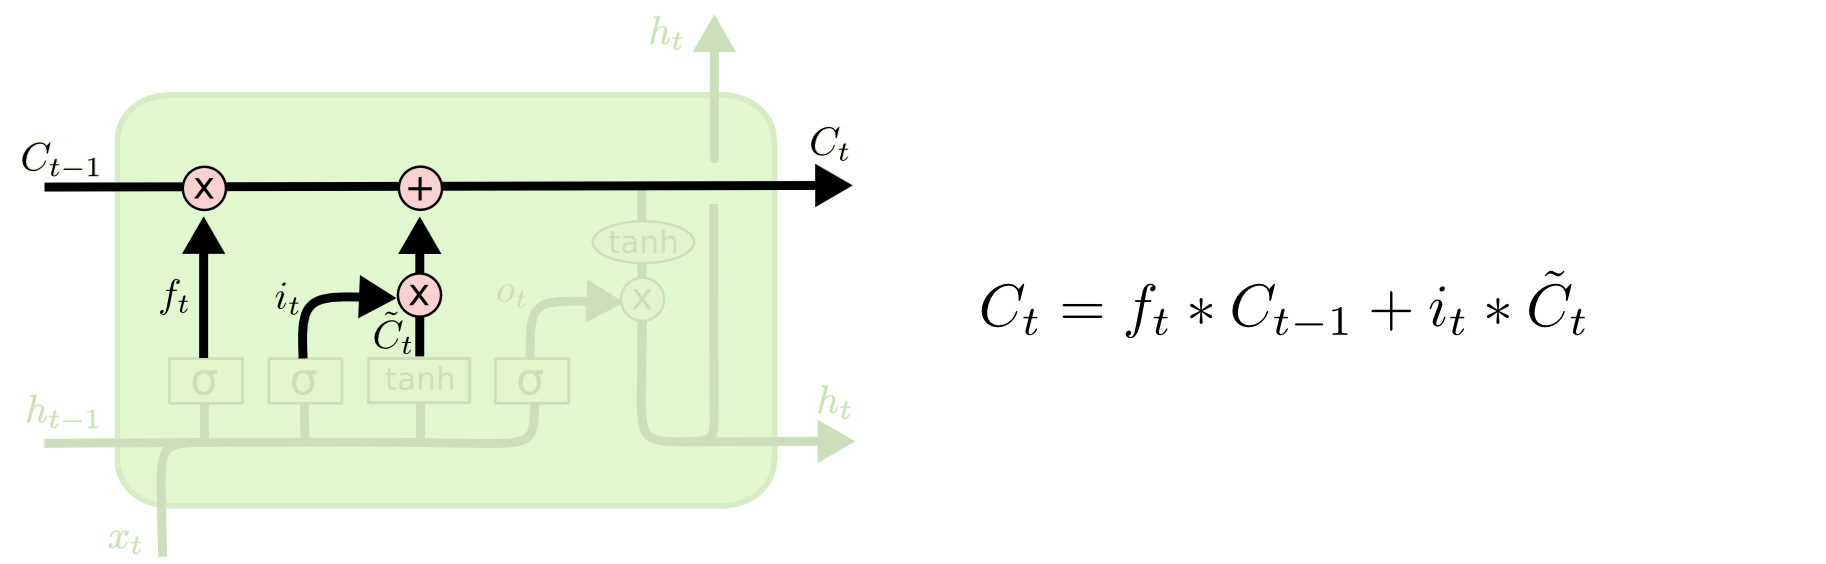
\includegraphics[width=0.85\textwidth]{rnn_lstm_03}
  \end{figure}

  \note{
    \begin{itemize}
      \item These parts of the candidate state are than added to the cell state.
      \item Image from Understanding LSTM Networks, Chris Olah\\
            \url{https://colah.github.io/posts/2015-08-Understanding-LSTMs/}
    \end{itemize}
  }
\end{frame}


\begin{frame}{Long Short Term Memory Networks}

  \begin{figure}
    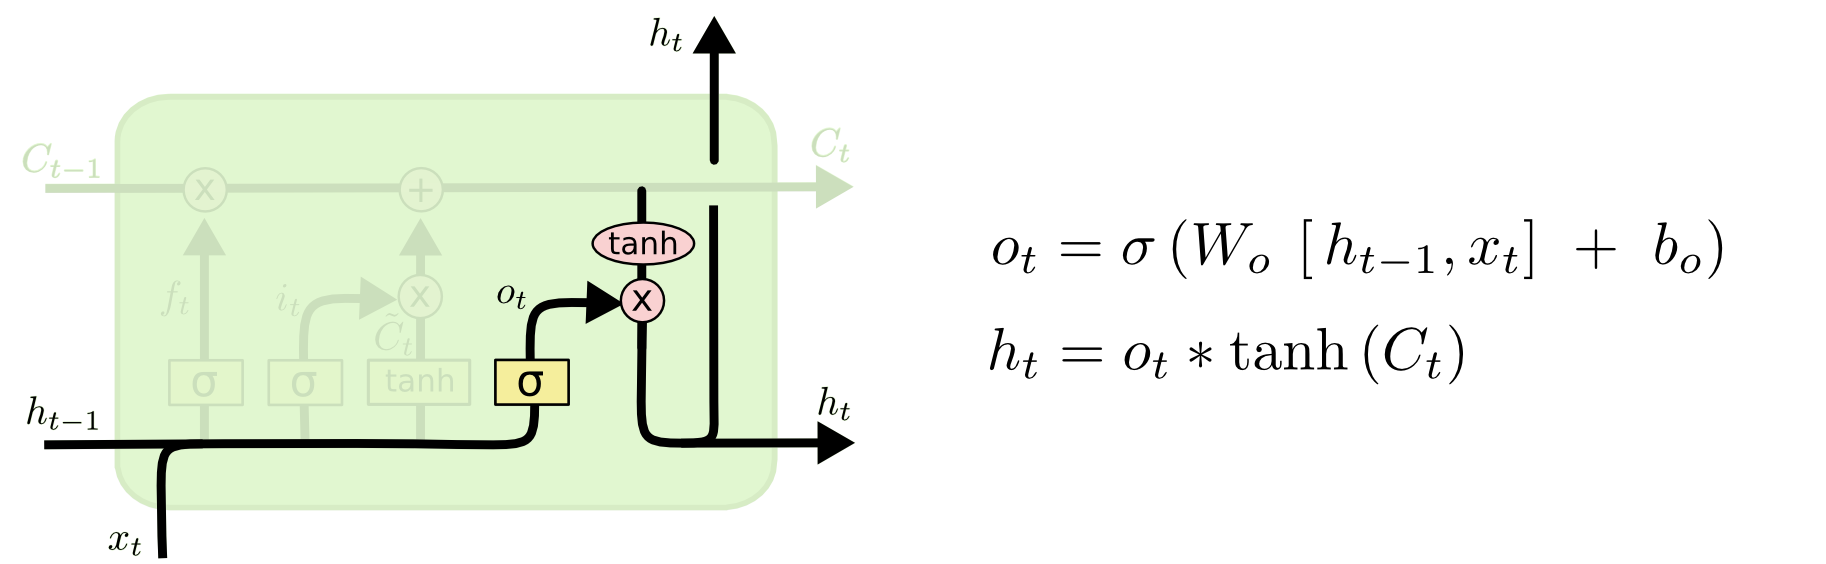
\includegraphics[width=0.85\textwidth]{rnn_lstm_04}
  \end{figure}

  \note{
    \begin{itemize}
      \item The output gate decides which parts of the cell state are going to be the output state.
      \item Image from Understanding LSTM Networks, Chris Olah\\
            \url{https://colah.github.io/posts/2015-08-Understanding-LSTMs/}
    \end{itemize}
  }
\end{frame}


\begin{frame}{Gated Recurrent Units}

  \begin{figure}
    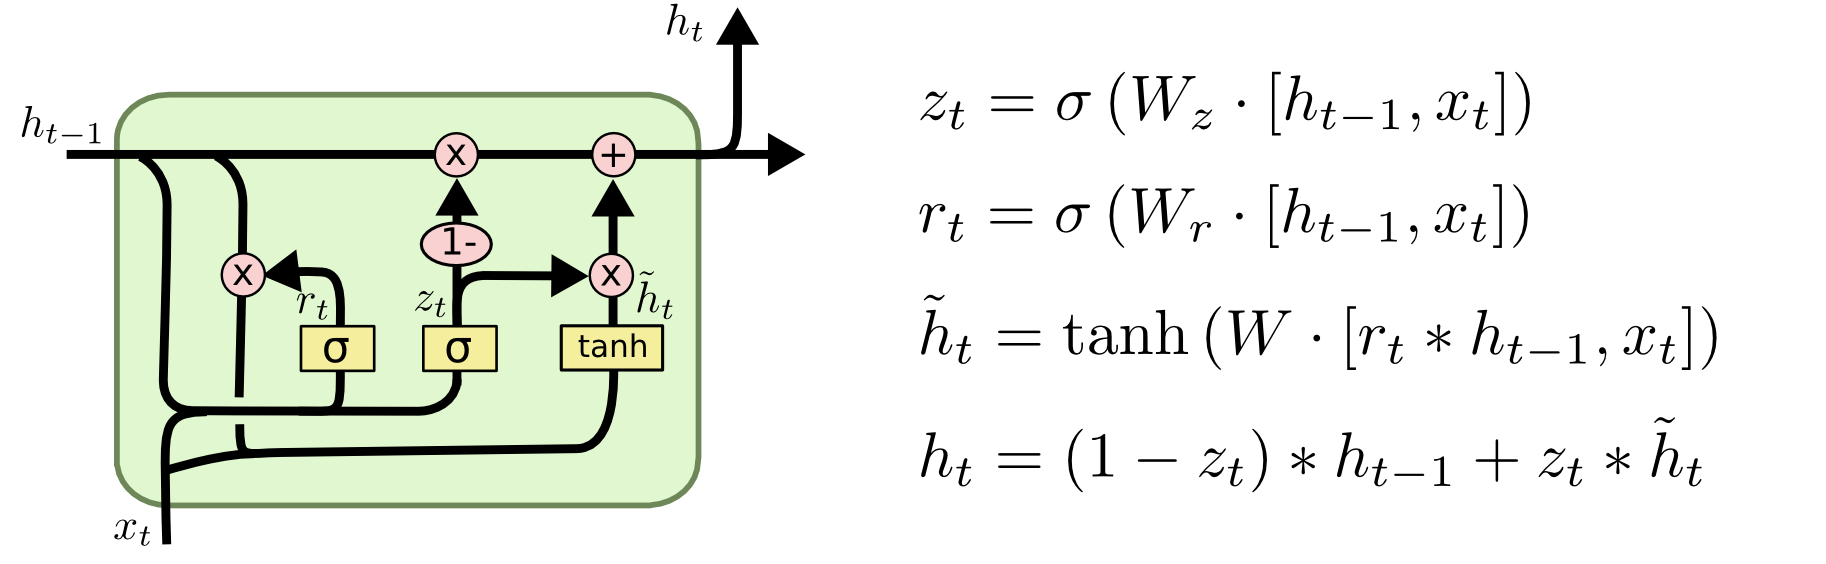
\includegraphics[width=0.85\textwidth]{rnn_gru_00}
  \end{figure}

  \note{
    \begin{itemize}
      \item Learning Phrase Representations using RNN Encoder–Decoder for Statistical Machine Translation, Cho et al., 2014
      \item GRUs combine the cell state and output and merge input and forget gate.
      \item Image from Understanding LSTM Networks, Chris Olah\\
            \url{https://colah.github.io/posts/2015-08-Understanding-LSTMs/}
    \end{itemize}
  }
\end{frame}


\begin{frame}{LSTM + Spatial encoder}

  \begin{figure}
    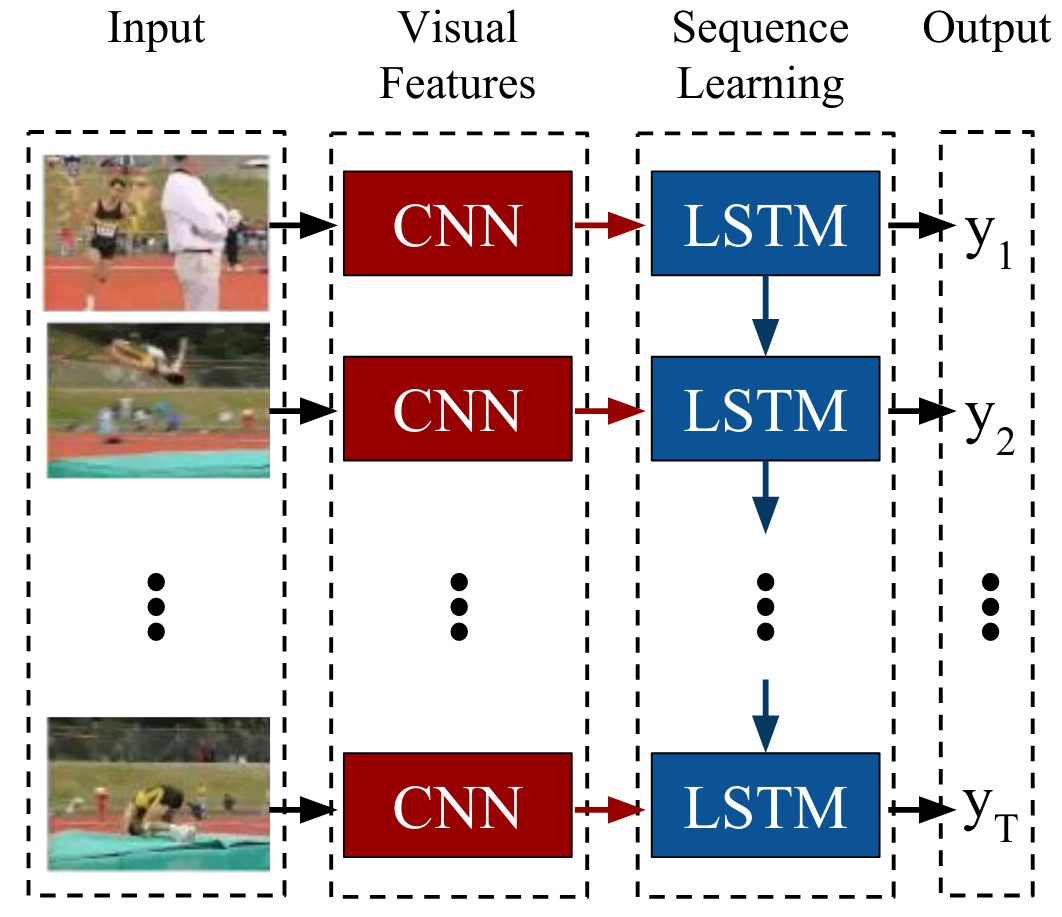
\includegraphics[width=0.65\textwidth]{lstmconv}
  \end{figure}

  \note{
    \begin{itemize}
      \item Image from Long-term Recurrent Convolutional Networks forVisual Recognition and Description, Donahue et al., CVPR 2015
    \end{itemize}
  }
\end{frame}


\begin{frame}{Stacked LSTM + Spatial encoder}

  \begin{figure}
    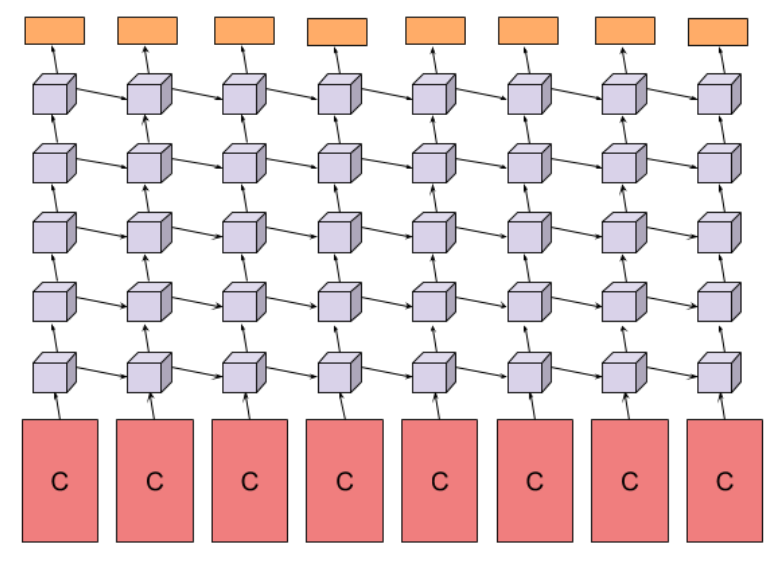
\includegraphics[width=0.65\textwidth]{stackedlstm}
  \end{figure}

  \note{
    \begin{itemize}
      \item Beyond Short Snippets: Deep Networks for Video Classification, Joe Yue-Hei Ng et al., CVPR 2015
    \end{itemize}
  }
\end{frame}



\begin{frame}{Convolutional LSTM}

  \begin{figure}
    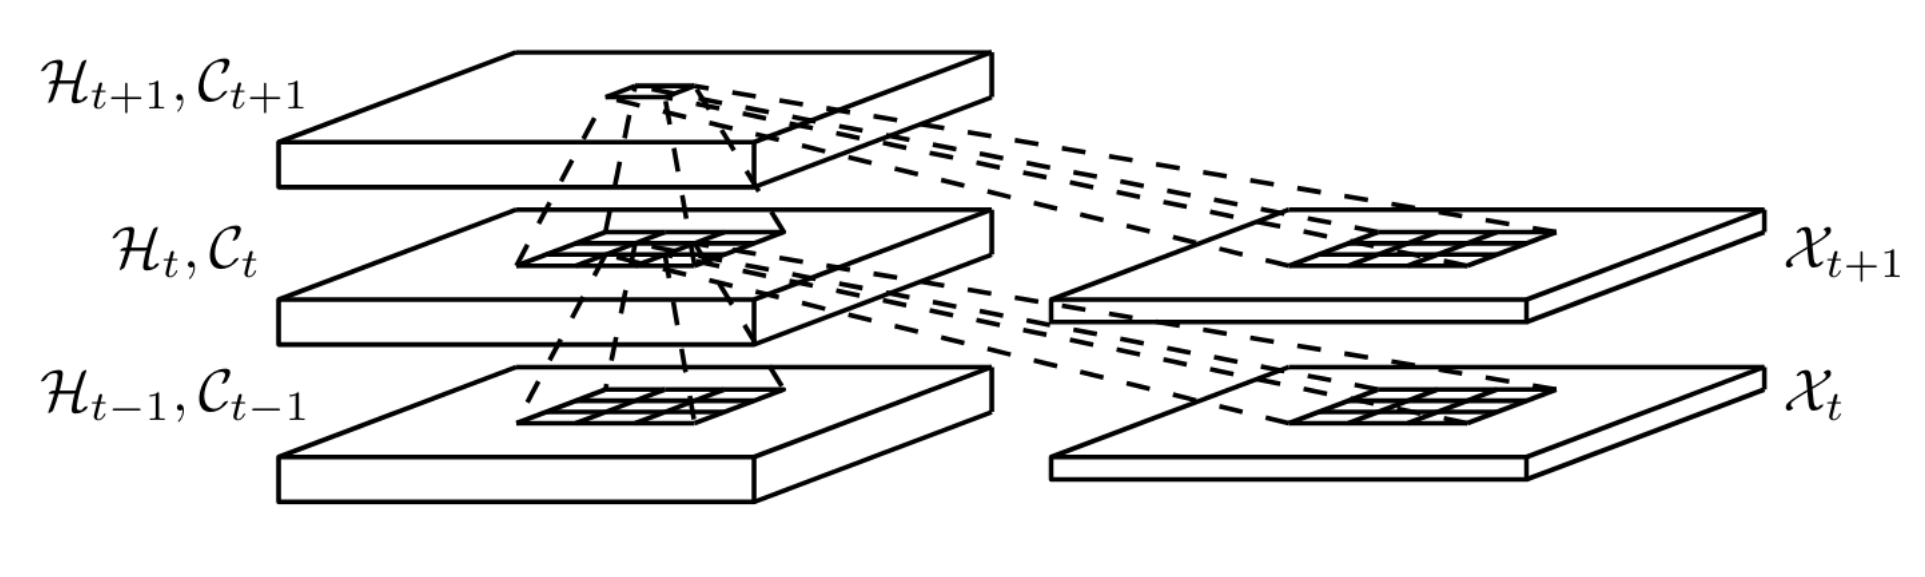
\includegraphics[width=0.65\textwidth]{convlstm}
  \end{figure}

  \note{
    \begin{itemize}
      \item
      \item Image from Convolutional LSTM Network: A Machine LearningApproach for Precipitation Nowcasting, Shi et al., 2015
    \end{itemize}
  }
\end{frame}


\begin{frame}{Convolutional LSTM + 3d convolutions}

  \begin{figure}
    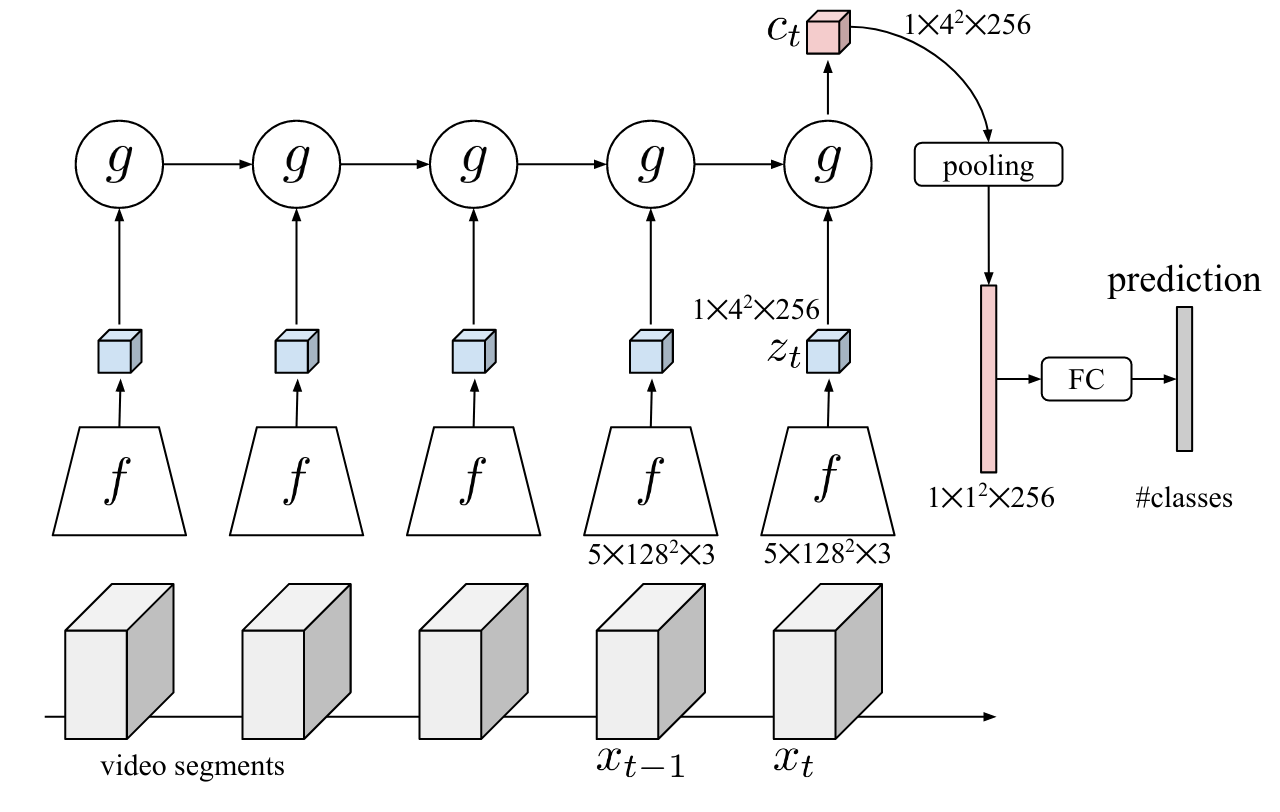
\includegraphics[width=0.65\textwidth]{3dconvlstm}
  \end{figure}

  \note{
    \begin{itemize}
      \item
      \item Video Representation Learning by Dense Predictive Coding, Han et al., ICCV 2019
    \end{itemize}
  }
\end{frame}


\begin{frame}{Sequence to Sequence}

  \begin{figure}
    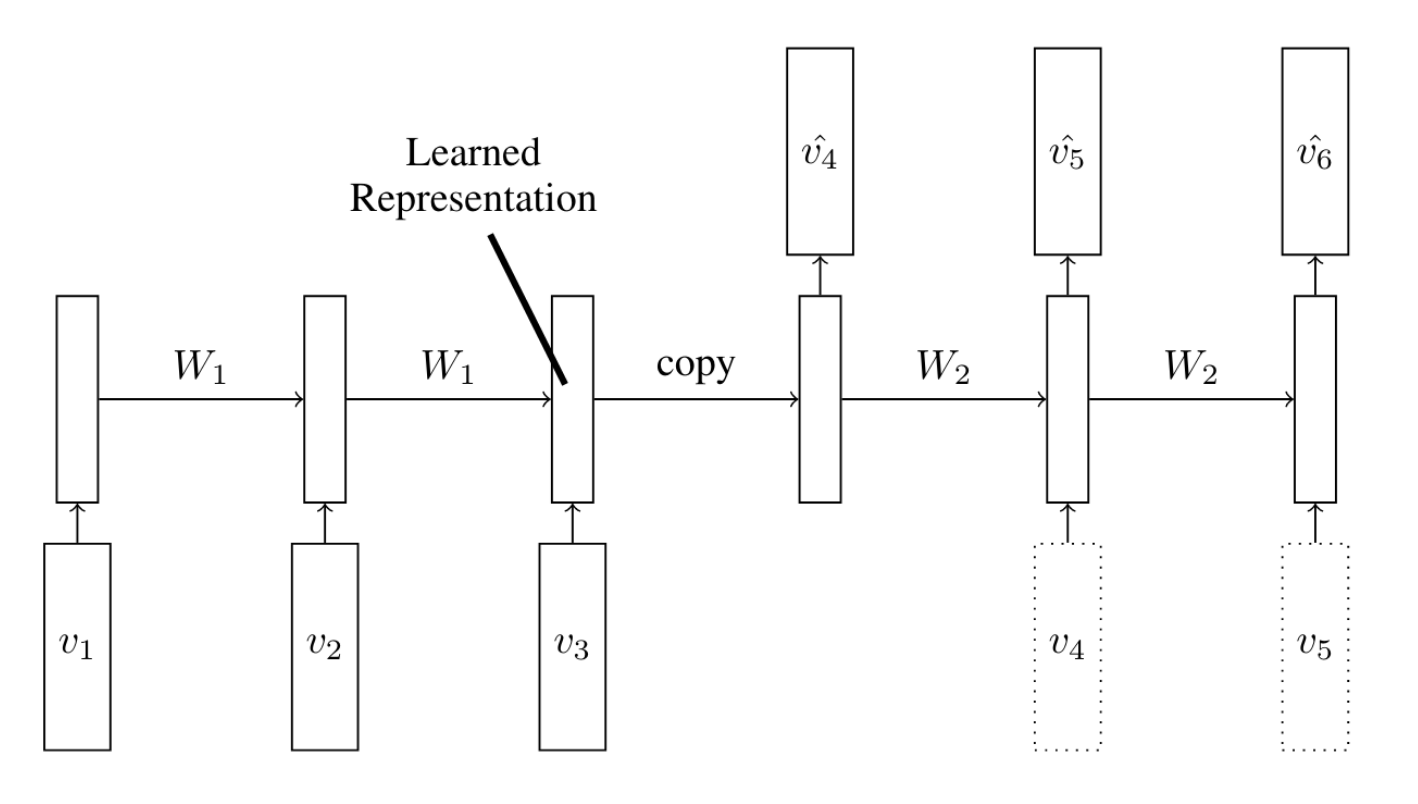
\includegraphics[width=0.65\textwidth]{predcoding}
  \end{figure}

  \note{
    \begin{itemize}
      \item Similar as in static images can be used for representation learning, video synthesis, style transfer, ...
      \item Image from Unsupervised Learning of Video Representations using LSTMs, Srivastava et al., 2015
    \end{itemize}
  }
\end{frame}


\begin{frame}{Mean Squared Future?}

  \begin{figure}
    
\includegraphics[width=0.45\textwidth]{cointoss}
  \end{figure}

  \note{
    \begin{itemize}
      \item Image from \url{https://commons.wikimedia.org/wiki/File:Coin_Toss_(3635981474).jpg}
      \item
    \end{itemize}
  }
\end{frame}


\begin{frame}{Mean Squared Future?}
  \begin{columns}
    \begin{column}{0.48\textwidth}
      \begin{figure}
        
\includegraphics[width=0.8\textwidth]{cointoss}
      \end{figure}
    \end{column}
    \begin{column}{0.48\textwidth}
    \begin{itemize}
      \item Probabilistic modeling
      \item Adversarial training
    \end{itemize}
    \end{column}
  \end{columns}

  \note{
    \begin{itemize}
      \item Image from \url{https://commons.wikimedia.org/wiki/File:Coin_Toss_(3635981474).jpg}
      \item
    \end{itemize}
  }
\end{frame}
